\documentclass[twoside]{book}

% Packages required by doxygen
\usepackage{fixltx2e}
\usepackage{calc}
\usepackage{doxygen}
\usepackage[export]{adjustbox} % also loads graphicx
\usepackage{graphicx}
\usepackage[utf8]{inputenc}
\usepackage{makeidx}
\usepackage{multicol}
\usepackage{multirow}
\PassOptionsToPackage{warn}{textcomp}
\usepackage{textcomp}
\usepackage[nointegrals]{wasysym}
\usepackage[table]{xcolor}

% Font selection
\usepackage[T1]{fontenc}
\usepackage[scaled=.90]{helvet}
\usepackage{courier}
\usepackage{amssymb}
\usepackage{sectsty}
\renewcommand{\familydefault}{\sfdefault}
\allsectionsfont{%
  \fontseries{bc}\selectfont%
  \color{darkgray}%
}
\renewcommand{\DoxyLabelFont}{%
  \fontseries{bc}\selectfont%
  \color{darkgray}%
}
\newcommand{\+}{\discretionary{\mbox{\scriptsize$\hookleftarrow$}}{}{}}

% Page & text layout
\usepackage{geometry}
\geometry{%
  a4paper,%
  top=2.5cm,%
  bottom=2.5cm,%
  left=2.5cm,%
  right=2.5cm%
}
\tolerance=750
\hfuzz=15pt
\hbadness=750
\setlength{\emergencystretch}{15pt}
\setlength{\parindent}{0cm}
\setlength{\parskip}{3ex plus 2ex minus 2ex}
\makeatletter
\renewcommand{\paragraph}{%
  \@startsection{paragraph}{4}{0ex}{-1.0ex}{1.0ex}{%
    \normalfont\normalsize\bfseries\SS@parafont%
  }%
}
\renewcommand{\subparagraph}{%
  \@startsection{subparagraph}{5}{0ex}{-1.0ex}{1.0ex}{%
    \normalfont\normalsize\bfseries\SS@subparafont%
  }%
}
\makeatother

% Headers & footers
\usepackage{fancyhdr}
\pagestyle{fancyplain}
\fancyhead[LE]{\fancyplain{}{\bfseries\thepage}}
\fancyhead[CE]{\fancyplain{}{}}
\fancyhead[RE]{\fancyplain{}{\bfseries\leftmark}}
\fancyhead[LO]{\fancyplain{}{\bfseries\rightmark}}
\fancyhead[CO]{\fancyplain{}{}}
\fancyhead[RO]{\fancyplain{}{\bfseries\thepage}}
\fancyfoot[LE]{\fancyplain{}{}}
\fancyfoot[CE]{\fancyplain{}{}}
\fancyfoot[RE]{\fancyplain{}{\bfseries\scriptsize Generated by Doxygen }}
\fancyfoot[LO]{\fancyplain{}{\bfseries\scriptsize Generated by Doxygen }}
\fancyfoot[CO]{\fancyplain{}{}}
\fancyfoot[RO]{\fancyplain{}{}}
\renewcommand{\footrulewidth}{0.4pt}
\renewcommand{\chaptermark}[1]{%
  \markboth{#1}{}%
}
\renewcommand{\sectionmark}[1]{%
  \markright{\thesection\ #1}%
}

% Indices & bibliography
\usepackage{natbib}
\usepackage[titles]{tocloft}
\setcounter{tocdepth}{3}
\setcounter{secnumdepth}{5}
\makeindex

% Hyperlinks (required, but should be loaded last)
\usepackage{ifpdf}
\ifpdf
  \usepackage[pdftex,pagebackref=true]{hyperref}
\else
  \usepackage[ps2pdf,pagebackref=true]{hyperref}
\fi
\hypersetup{%
  colorlinks=true,%
  linkcolor=blue,%
  citecolor=blue,%
  unicode%
}

% Custom commands
\newcommand{\clearemptydoublepage}{%
  \newpage{\pagestyle{empty}\cleardoublepage}%
}

\usepackage{caption}
\captionsetup{labelsep=space,justification=centering,font={bf},singlelinecheck=off,skip=4pt,position=top}

%===== C O N T E N T S =====

\begin{document}

% Titlepage & ToC
\hypersetup{pageanchor=false,
             bookmarksnumbered=true,
             pdfencoding=unicode
            }
\pagenumbering{alph}
\begin{titlepage}
\vspace*{7cm}
\begin{center}%
{\Large Open\+GL Spectrogram \\[1ex]\large 1.\+1 }\\
\vspace*{1cm}
{\large Generated by Doxygen 1.8.14}\\
\end{center}
\end{titlepage}
\clearemptydoublepage
\pagenumbering{roman}
\tableofcontents
\clearemptydoublepage
\pagenumbering{arabic}
\hypersetup{pageanchor=true}

%--- Begin generated contents ---
\chapter{Hierarchical Index}
\section{Class Hierarchy}
This inheritance list is sorted roughly, but not completely, alphabetically\+:\begin{DoxyCompactList}
\item \contentsline{section}{Audio\+Input}{\pageref{classAudioInput}}{}
\begin{DoxyCompactList}
\item \contentsline{section}{A\+L\+SA}{\pageref{classALSA}}{}
\end{DoxyCompactList}
\item \contentsline{section}{Display}{\pageref{classDisplay}}{}
\item \contentsline{section}{Graphics\+Item}{\pageref{classGraphicsItem}}{}
\begin{DoxyCompactList}
\item \contentsline{section}{Spectrogram\+Visualizer}{\pageref{structSpectrogramVisualizer}}{}
\end{DoxyCompactList}
\item K\+E\+Y\+B\+O\+A\+R\+D\+\_\+\+S\+H\+O\+R\+T\+C\+U\+TS\begin{DoxyCompactList}
\item \contentsline{section}{Spectrogram\+Visualizer}{\pageref{structSpectrogramVisualizer}}{}
\end{DoxyCompactList}
\item \contentsline{section}{Log}{\pageref{classLog}}{}
\item \contentsline{section}{Param}{\pageref{structParam}}{}
\item \contentsline{section}{Spectrogram\+Visualizer\+:\+:shortcuts}{\pageref{structSpectrogramVisualizer_1_1shortcuts}}{}
\end{DoxyCompactList}

\chapter{Class Index}
\section{Class List}
Here are the classes, structs, unions and interfaces with brief descriptions\+:\begin{DoxyCompactList}
\item\contentsline{section}{\hyperlink{classALSA}{A\+L\+SA} }{\pageref{classALSA}}{}
\item\contentsline{section}{\hyperlink{classAudioInput}{Audio\+Input} }{\pageref{classAudioInput}}{}
\item\contentsline{section}{\hyperlink{classDisplay}{Display} }{\pageref{classDisplay}}{}
\item\contentsline{section}{\hyperlink{classGraphicsItem}{Graphics\+Item} }{\pageref{classGraphicsItem}}{}
\item\contentsline{section}{\hyperlink{classLog}{Log} }{\pageref{classLog}}{}
\item\contentsline{section}{\hyperlink{structParam}{Param} }{\pageref{structParam}}{}
\item\contentsline{section}{\hyperlink{structSpectrogramVisualizer_1_1shortcuts}{Spectrogram\+Visualizer\+::shortcuts} }{\pageref{structSpectrogramVisualizer_1_1shortcuts}}{}
\item\contentsline{section}{\hyperlink{structSpectrogramVisualizer}{Spectrogram\+Visualizer} }{\pageref{structSpectrogramVisualizer}}{}
\end{DoxyCompactList}

\chapter{Class Documentation}
\hypertarget{classAudioInput}{}\section{Audio\+Input Class Reference}
\label{classAudioInput}\index{Audio\+Input@{Audio\+Input}}


{\ttfamily \#include $<$Audio\+Input.\+hpp$>$}

Inheritance diagram for Audio\+Input\+:\begin{figure}[H]
\begin{center}
\leavevmode
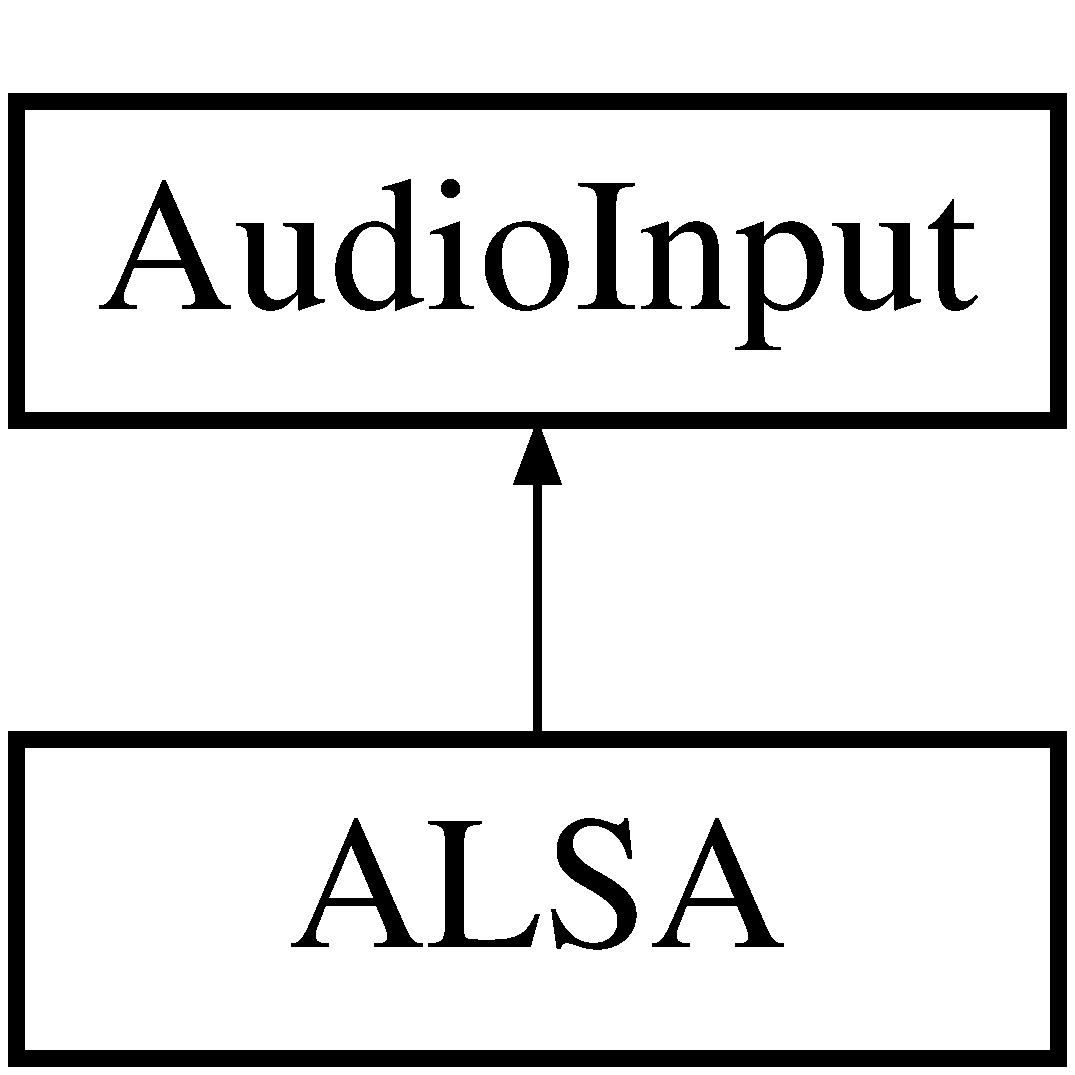
\includegraphics[height=2.000000cm]{classAudioInput}
\end{center}
\end{figure}
\subsection*{Public Member Functions}
\begin{DoxyCompactItemize}
\item 
\mbox{\hyperlink{classAudioInput_a51903411fbfb29b77f30a0ee3fbaa50e}{Audio\+Input}} ()
\item 
\mbox{\Hypertarget{classAudioInput_a8a86507eb41c9db581def690f1f96669}\label{classAudioInput_a8a86507eb41c9db581def690f1f96669}} 
{\bfseries Audio\+Input} (const \mbox{\hyperlink{classAudioInput}{Audio\+Input}} \&)
\item 
\mbox{\Hypertarget{classAudioInput_a104f135fc060ebd133166516650304e0}\label{classAudioInput_a104f135fc060ebd133166516650304e0}} 
\mbox{\hyperlink{classAudioInput}{Audio\+Input}} \& {\bfseries operator=} (const \mbox{\hyperlink{classAudioInput}{Audio\+Input}} \&)
\item 
virtual \mbox{\hyperlink{classAudioInput_aaf278510da0fee4ccfd44c679067d96c}{$\sim$\+Audio\+Input}} ()=0
\item 
void \mbox{\hyperlink{classAudioInput_abe6c5796db5f1f0d4944a3c9e8b3962e}{initialize\+Window}} (float $\ast$window, int window\+Size, unsigned int window\+Type)
\item 
virtual void \mbox{\hyperlink{classAudioInput_a4fce5476455b1df813f1cb6eebb08311}{quit\+Now}} ()=0
\item 
virtual int \mbox{\hyperlink{classAudioInput_afa753742035f7069f5ef0c2ece6a62fe}{start\+Capture}} ()=0
\item 
\mbox{\Hypertarget{classAudioInput_ae877bcc482868235b38fc7bb099d7a43}\label{classAudioInput_ae877bcc482868235b38fc7bb099d7a43}} 
unsigned long {\bfseries get\+Buffer\+Size\+Frames} () const
\item 
\mbox{\Hypertarget{classAudioInput_a30068a991c436282680a320c043d021f}\label{classAudioInput_a30068a991c436282680a320c043d021f}} 
void {\bfseries set\+Buffer\+Size\+Frames} (unsigned long \mbox{\hyperlink{classAudioInput_adb734d274b7ce2967b74e2280ff6d487}{buffer\+Size\+Frames}})
\item 
\mbox{\Hypertarget{classAudioInput_a9a6e1385e3bc495fca357ab684301daa}\label{classAudioInput_a9a6e1385e3bc495fca357ab684301daa}} 
int {\bfseries get\+Buffer\+Size\+Samples} () const
\item 
\mbox{\Hypertarget{classAudioInput_a23e782296cc43ff127d9f95f77902b94}\label{classAudioInput_a23e782296cc43ff127d9f95f77902b94}} 
void {\bfseries set\+Buffer\+Size\+Samples} (int \mbox{\hyperlink{classAudioInput_a4e213a9a22a62dccc3a54369101559c7}{buffer\+Size\+Samples}})
\item 
\mbox{\Hypertarget{classAudioInput_ac56e6ce779b652bd8fc343828a40fe76}\label{classAudioInput_ac56e6ce779b652bd8fc343828a40fe76}} 
float $\ast$ {\bfseries get\+Audio\+Buffer} () const
\item 
\mbox{\Hypertarget{classAudioInput_a33e4d0a312cc8f3c26f0f06c9bee9fd8}\label{classAudioInput_a33e4d0a312cc8f3c26f0f06c9bee9fd8}} 
void {\bfseries set\+Audio\+Buffer} (float $\ast$\mbox{\hyperlink{classAudioInput_a797943485896a381ea80947c8b6a8488}{audio\+Buffer}})
\item 
\mbox{\Hypertarget{classAudioInput_a407e9626c0ab056dd0d4401ce5056d00}\label{classAudioInput_a407e9626c0ab056dd0d4401ce5056d00}} 
float $\ast$ {\bfseries get\+Spectrogram\+Slice} () const
\item 
\mbox{\Hypertarget{classAudioInput_a55f5b0061a542195af4161c5ef931d2b}\label{classAudioInput_a55f5b0061a542195af4161c5ef931d2b}} 
void {\bfseries set\+Spectrogram\+Slice} (float $\ast$\mbox{\hyperlink{classAudioInput_aa277accc3be5054fe8439ac7086deaf5}{spectrogram\+Slice}})
\item 
\mbox{\Hypertarget{classAudioInput_ac7a550e7e3d4312b576978df832d70ec}\label{classAudioInput_ac7a550e7e3d4312b576978df832d70ec}} 
float $\ast$ {\bfseries get\+Windowing\+Function} () const
\item 
\mbox{\Hypertarget{classAudioInput_a4c11f1a37408349ee4d7354e1c2fdd11}\label{classAudioInput_a4c11f1a37408349ee4d7354e1c2fdd11}} 
void {\bfseries set\+Windowing\+Function} (float $\ast$\mbox{\hyperlink{classAudioInput_a72417120c208d81359f5b1205fc06664}{windowing\+Function}})
\item 
\mbox{\Hypertarget{classAudioInput_afa340ece9b45d8d4bb85972edfe9712b}\label{classAudioInput_afa340ece9b45d8d4bb85972edfe9712b}} 
unsigned int {\bfseries get\+Spectrogram\+Size} () const
\item 
\mbox{\Hypertarget{classAudioInput_a900f80fe37d48bc77d99cc0971f01ea7}\label{classAudioInput_a900f80fe37d48bc77d99cc0971f01ea7}} 
void {\bfseries set\+Spectrogram\+Size} (unsigned int \mbox{\hyperlink{classAudioInput_a1d4982a84d2e2e3d8a6b0f0fcdd4820e}{spectrogram\+Size}})
\item 
\mbox{\Hypertarget{classAudioInput_a069f76d3553328428959325c1be3ee3e}\label{classAudioInput_a069f76d3553328428959325c1be3ee3e}} 
unsigned int {\bfseries get\+Fft\+Length} () const
\item 
\mbox{\Hypertarget{classAudioInput_a71e1759bc4267b436bd9b4b8937dcabd}\label{classAudioInput_a71e1759bc4267b436bd9b4b8937dcabd}} 
void {\bfseries set\+Fft\+Length} (unsigned int \mbox{\hyperlink{classAudioInput_a5b31598e9106da62d86d11d69a9dbd20}{fft\+Length}})
\item 
\mbox{\Hypertarget{classAudioInput_a547f6144fe074436c678776f647dcf02}\label{classAudioInput_a547f6144fe074436c678776f647dcf02}} 
float {\bfseries get\+Buffer\+Memory\+Seconds} () const
\item 
\mbox{\Hypertarget{classAudioInput_a2ac6cfeb9f0d289cb5170d03a07472ef}\label{classAudioInput_a2ac6cfeb9f0d289cb5170d03a07472ef}} 
void {\bfseries set\+Buffer\+Memory\+Seconds} (float \mbox{\hyperlink{classAudioInput_aea3145ccca0f7cebf36a78278ca44031}{buffer\+Memory\+Seconds}})
\item 
\mbox{\Hypertarget{classAudioInput_a2b531eed74caeceff65deed019976804}\label{classAudioInput_a2b531eed74caeceff65deed019976804}} 
unsigned int {\bfseries get\+N\+Channels} () const
\item 
\mbox{\Hypertarget{classAudioInput_a3f4482ac752d8028e433e9543a53a83a}\label{classAudioInput_a3f4482ac752d8028e433e9543a53a83a}} 
void {\bfseries set\+N\+Channels} (unsigned int \mbox{\hyperlink{classAudioInput_a364801e7fa59b6c8ed881262b2085d42}{n\+Channels}})
\item 
\mbox{\Hypertarget{classAudioInput_a261c017ca0b89a14ff0e0119bea6d8bd}\label{classAudioInput_a261c017ca0b89a14ff0e0119bea6d8bd}} 
float {\bfseries get\+Sampling\+Period} () const
\item 
\mbox{\Hypertarget{classAudioInput_afbac34c42a21c102cb0c9f8db9083da5}\label{classAudioInput_afbac34c42a21c102cb0c9f8db9083da5}} 
void {\bfseries set\+Sampling\+Period} (float \mbox{\hyperlink{classAudioInput_a8b6ea4cd6b88e5cd9d051b298efbb65e}{sampling\+Period}})
\item 
\mbox{\Hypertarget{classAudioInput_afeef426fc67f34a73132955f72068266}\label{classAudioInput_afeef426fc67f34a73132955f72068266}} 
bool {\bfseries is\+Quit} () const
\item 
\mbox{\Hypertarget{classAudioInput_af5c79f83c5e014bdf12d3ad623e65be5}\label{classAudioInput_af5c79f83c5e014bdf12d3ad623e65be5}} 
void {\bfseries set\+Quit} (bool \mbox{\hyperlink{classAudioInput_aceef1c12e4f78624ed695371adf495df}{quit}})
\item 
\mbox{\Hypertarget{classAudioInput_a59df92ca184977f5a400fe6d5cea33fc}\label{classAudioInput_a59df92ca184977f5a400fe6d5cea33fc}} 
bool {\bfseries is\+Pause} () const
\item 
\mbox{\Hypertarget{classAudioInput_abc3f83d5ce04a9628bcf658cc857d786}\label{classAudioInput_abc3f83d5ce04a9628bcf658cc857d786}} 
void {\bfseries set\+Pause} (bool \mbox{\hyperlink{classAudioInput_a3ff41f73529f77872f6ab585d7cf706a}{pause}})
\item 
\mbox{\Hypertarget{classAudioInput_a19c4e0c35b8360b0dca9cf5cad3d2e64}\label{classAudioInput_a19c4e0c35b8360b0dca9cf5cad3d2e64}} 
unsigned int {\bfseries get\+Sampling\+Rate} () const
\item 
\mbox{\Hypertarget{classAudioInput_a621a6d87ca463668289f2cb7fa97c75c}\label{classAudioInput_a621a6d87ca463668289f2cb7fa97c75c}} 
void {\bfseries set\+Sampling\+Rate} (unsigned int \mbox{\hyperlink{classAudioInput_acfe371c4f5790bd67d282bc83225728e}{sampling\+Rate}})
\item 
\mbox{\Hypertarget{classAudioInput_a78df439ada22ba00be19c4c8a82bbe3d}\label{classAudioInput_a78df439ada22ba00be19c4c8a82bbe3d}} 
int {\bfseries get\+Buffer\+Index} () const
\item 
\mbox{\Hypertarget{classAudioInput_a506d7f5eec641d0232286ea145270038}\label{classAudioInput_a506d7f5eec641d0232286ea145270038}} 
void {\bfseries set\+Buffer\+Index} (int \mbox{\hyperlink{classAudioInput_a3c9888a90ca8bc6b42257f3f11ee9a6e}{buffer\+Index}})
\item 
\mbox{\Hypertarget{classAudioInput_a4de4a846fe48603932495acaafc54449}\label{classAudioInput_a4de4a846fe48603932495acaafc54449}} 
float $\ast$ {\bfseries get\+Windowed\+Audio\+Frame} () const
\item 
\mbox{\Hypertarget{classAudioInput_a8e7dd67ab635c3935bd54f72a5282dce}\label{classAudioInput_a8e7dd67ab635c3935bd54f72a5282dce}} 
void {\bfseries set\+Windowed\+Audio\+Frame} (float $\ast$\mbox{\hyperlink{classAudioInput_ae5a196a9ba111b7aa1ef64db6f092432}{windowed\+Audio\+Frame}})
\end{DoxyCompactItemize}
\subsection*{Static Public Member Functions}
\begin{DoxyCompactItemize}
\item 
static void \mbox{\hyperlink{classAudioInput_a77614769e39be88bbf5d78adf84d9260}{compute\+Spectrogram\+Slice}} (\mbox{\hyperlink{classAudioInput}{Audio\+Input}} $\ast$audio\+Input)
\item 
static const unsigned int \mbox{\hyperlink{classAudioInput_a76a26e018987d0a303a32852ebf85254}{get\+V\+E\+R\+B\+O\+S\+I\+TY}} ()
\item 
\mbox{\Hypertarget{classAudioInput_ae73b1fc55b3247b431d27bb673318dde}\label{classAudioInput_ae73b1fc55b3247b431d27bb673318dde}} 
static const unsigned int {\bfseries get\+N\+\_\+\+F\+R\+E\+Q\+U\+E\+N\+C\+I\+ES} ()
\item 
\mbox{\Hypertarget{classAudioInput_a6e33130e47360bad95cfeb094f079334}\label{classAudioInput_a6e33130e47360bad95cfeb094f079334}} 
static const unsigned int {\bfseries get\+N\+\_\+\+T\+I\+M\+E\+\_\+\+W\+I\+N\+D\+O\+WS} ()
\end{DoxyCompactItemize}
\subsection*{Static Public Attributes}
\begin{DoxyCompactItemize}
\item 
static const unsigned int \mbox{\hyperlink{classAudioInput_aff0f7df20d558ba13f85b3d49b7f42b2}{V\+E\+R\+B\+O\+S\+I\+TY}} = 2
\item 
static const unsigned int \mbox{\hyperlink{classAudioInput_a4be6c19fca6626b2ccee1eeca458f7c8}{N\+\_\+\+F\+R\+E\+Q\+U\+E\+N\+C\+I\+ES}} = 2048
\item 
static const unsigned int \mbox{\hyperlink{classAudioInput_a8b6b39b0558d7db54234f1e39a38a775}{N\+\_\+\+T\+I\+M\+E\+\_\+\+W\+I\+N\+D\+O\+WS}} = 940
\end{DoxyCompactItemize}
\subsection*{Protected Attributes}
\begin{DoxyCompactItemize}
\item 
unsigned long \mbox{\hyperlink{classAudioInput_adb734d274b7ce2967b74e2280ff6d487}{buffer\+Size\+Frames}}
\item 
int \mbox{\hyperlink{classAudioInput_a4e213a9a22a62dccc3a54369101559c7}{buffer\+Size\+Samples}}
\item 
float $\ast$ \mbox{\hyperlink{classAudioInput_a797943485896a381ea80947c8b6a8488}{audio\+Buffer}}
\item 
int \mbox{\hyperlink{classAudioInput_a3c9888a90ca8bc6b42257f3f11ee9a6e}{buffer\+Index}}
\item 
float $\ast$ \mbox{\hyperlink{classAudioInput_aa277accc3be5054fe8439ac7086deaf5}{spectrogram\+Slice}}
\item 
float $\ast$ \mbox{\hyperlink{classAudioInput_a72417120c208d81359f5b1205fc06664}{windowing\+Function}}
\item 
float $\ast$ \mbox{\hyperlink{classAudioInput_a0c0e5c44a1547a97564e0733aaac2dc0}{fft\+Frame}}
\item 
float $\ast$ \mbox{\hyperlink{classAudioInput_ae5a196a9ba111b7aa1ef64db6f092432}{windowed\+Audio\+Frame}}
\item 
unsigned int \mbox{\hyperlink{classAudioInput_a1d4982a84d2e2e3d8a6b0f0fcdd4820e}{spectrogram\+Size}}
\item 
unsigned int \mbox{\hyperlink{classAudioInput_a5b31598e9106da62d86d11d69a9dbd20}{fft\+Length}}
\item 
float \mbox{\hyperlink{classAudioInput_aea3145ccca0f7cebf36a78278ca44031}{buffer\+Memory\+Seconds}}
\item 
unsigned int \mbox{\hyperlink{classAudioInput_a364801e7fa59b6c8ed881262b2085d42}{n\+Channels}}
\item 
unsigned int \mbox{\hyperlink{classAudioInput_acfe371c4f5790bd67d282bc83225728e}{sampling\+Rate}}
\item 
float \mbox{\hyperlink{classAudioInput_a8b6ea4cd6b88e5cd9d051b298efbb65e}{sampling\+Period}}
\item 
bool \mbox{\hyperlink{classAudioInput_aceef1c12e4f78624ed695371adf495df}{quit}}
\item 
bool \mbox{\hyperlink{classAudioInput_a3ff41f73529f77872f6ab585d7cf706a}{pause}}
\item 
fftwf\+\_\+plan \mbox{\hyperlink{classAudioInput_a9797094e75625173beae7e89497248b2}{fft\+Plan}}
\end{DoxyCompactItemize}


\subsection{Detailed Description}
Generic interface to obtaining audio input. \begin{DoxyAuthor}{Author}
Anthony Agnone, Aug 2016
\end{DoxyAuthor}
T\+O\+DO generalize to audio input or output. T\+O\+DO obtain shared verbosity indicator. T\+O\+DO obtain parameters from command-\/line. 

Definition at line 22 of file Audio\+Input.\+hpp.



\subsection{Constructor \& Destructor Documentation}
\mbox{\Hypertarget{classAudioInput_a51903411fbfb29b77f30a0ee3fbaa50e}\label{classAudioInput_a51903411fbfb29b77f30a0ee3fbaa50e}} 
\index{Audio\+Input@{Audio\+Input}!Audio\+Input@{Audio\+Input}}
\index{Audio\+Input@{Audio\+Input}!Audio\+Input@{Audio\+Input}}
\subsubsection{\texorpdfstring{Audio\+Input()}{AudioInput()}}
{\footnotesize\ttfamily Audio\+Input\+::\+Audio\+Input (\begin{DoxyParamCaption}{ }\end{DoxyParamCaption})}

Overloaded constructor to initialize various member parameters. 

Definition at line 9 of file Audio\+Input.\+cpp.


\begin{DoxyCode}
9                        \{
10     \mbox{\hyperlink{classAudioInput_aceef1c12e4f78624ed695371adf495df}{quit}} = \textcolor{keyword}{false};
11     \mbox{\hyperlink{classAudioInput_a3ff41f73529f77872f6ab585d7cf706a}{pause}} = \textcolor{keyword}{false};
12 
13     \mbox{\hyperlink{classAudioInput_a3c9888a90ca8bc6b42257f3f11ee9a6e}{bufferIndex}} = -2;
14 
15     \textcolor{comment}{// TODO change how class receives value for windowSizeExponent}
16     \textcolor{keywordtype}{unsigned} \textcolor{keywordtype}{int} twowinsize = 12;
17     \mbox{\hyperlink{classAudioInput_a5b31598e9106da62d86d11d69a9dbd20}{fftLength}} = (\textcolor{keywordtype}{unsigned} int) 1 << twowinsize;
18     \mbox{\hyperlink{classLog_a987f3ff401eea783d0e80daaea1d7aca}{Log::getInstance}}()->\mbox{\hyperlink{classLog_a32d048a4924c7851c4b7b16758675af6}{logger}}() << \textcolor{stringliteral}{"FFT Length: "} << 
      \mbox{\hyperlink{classAudioInput_a5b31598e9106da62d86d11d69a9dbd20}{fftLength}} << std::endl;
19     \mbox{\hyperlink{classAudioInput_ae5a196a9ba111b7aa1ef64db6f092432}{windowedAudioFrame}} = \textcolor{keyword}{new} \textcolor{keywordtype}{float}[\mbox{\hyperlink{classAudioInput_a5b31598e9106da62d86d11d69a9dbd20}{fftLength}}];
20     \mbox{\hyperlink{classAudioInput_a0c0e5c44a1547a97564e0733aaac2dc0}{fftFrame}} = \textcolor{keyword}{new} \textcolor{keywordtype}{float}[\mbox{\hyperlink{classAudioInput_a5b31598e9106da62d86d11d69a9dbd20}{fftLength}}];
21     \mbox{\hyperlink{classAudioInput_a72417120c208d81359f5b1205fc06664}{windowingFunction}} = \textcolor{keyword}{new} \textcolor{keywordtype}{float}[\mbox{\hyperlink{classAudioInput_a5b31598e9106da62d86d11d69a9dbd20}{fftLength}}];
22     \mbox{\hyperlink{classAudioInput_abe6c5796db5f1f0d4944a3c9e8b3962e}{initializeWindow}}(\mbox{\hyperlink{classAudioInput_a72417120c208d81359f5b1205fc06664}{windowingFunction}}, 
      \mbox{\hyperlink{classAudioInput_a5b31598e9106da62d86d11d69a9dbd20}{fftLength}}, 2);
23 
24     \textcolor{comment}{/* set up in-place single-precision real-to-half-complex FFT */}
25     \mbox{\hyperlink{classAudioInput_a9797094e75625173beae7e89497248b2}{fftPlan}} = fftwf\_plan\_r2r\_1d(\mbox{\hyperlink{classAudioInput_a5b31598e9106da62d86d11d69a9dbd20}{fftLength}}, \mbox{\hyperlink{classAudioInput_ae5a196a9ba111b7aa1ef64db6f092432}{windowedAudioFrame}}, 
      \mbox{\hyperlink{classAudioInput_a0c0e5c44a1547a97564e0733aaac2dc0}{fftFrame}}, FFTW\_R2HC, FFTW\_MEASURE);
26     \mbox{\hyperlink{classAudioInput_aa277accc3be5054fe8439ac7086deaf5}{spectrogramSlice}} = \textcolor{keyword}{new} \textcolor{keywordtype}{float}[\mbox{\hyperlink{classAudioInput_a4be6c19fca6626b2ccee1eeca458f7c8}{N\_FREQUENCIES}}];
27     \mbox{\hyperlink{classAudioInput_a1d4982a84d2e2e3d8a6b0f0fcdd4820e}{spectrogramSize}} = \mbox{\hyperlink{classAudioInput_a4be6c19fca6626b2ccee1eeca458f7c8}{N\_FREQUENCIES}} * \mbox{\hyperlink{classAudioInput_a8b6b39b0558d7db54234f1e39a38a775}{N\_TIME\_WINDOWS}};
28     \mbox{\hyperlink{classLog_a987f3ff401eea783d0e80daaea1d7aca}{Log::getInstance}}()->\mbox{\hyperlink{classLog_a32d048a4924c7851c4b7b16758675af6}{logger}}() << \textcolor{stringliteral}{"Finished creating AudioInput"} << std::endl;
29 \}
\end{DoxyCode}
\mbox{\Hypertarget{classAudioInput_aaf278510da0fee4ccfd44c679067d96c}\label{classAudioInput_aaf278510da0fee4ccfd44c679067d96c}} 
\index{Audio\+Input@{Audio\+Input}!````~Audio\+Input@{$\sim$\+Audio\+Input}}
\index{````~Audio\+Input@{$\sim$\+Audio\+Input}!Audio\+Input@{Audio\+Input}}
\subsubsection{\texorpdfstring{$\sim$\+Audio\+Input()}{~AudioInput()}}
{\footnotesize\ttfamily Audio\+Input\+::$\sim$\+Audio\+Input (\begin{DoxyParamCaption}{ }\end{DoxyParamCaption})\hspace{0.3cm}{\ttfamily [pure virtual]}}

Destructor de-\/allocates all dynamic memory and joins the audio retrieval thread. 

Definition at line 91 of file Audio\+Input.\+cpp.


\begin{DoxyCode}
91                         \{
92     fftwf\_destroy\_plan(\mbox{\hyperlink{classAudioInput_a9797094e75625173beae7e89497248b2}{fftPlan}});
93     \textcolor{keyword}{delete}[] \mbox{\hyperlink{classAudioInput_a797943485896a381ea80947c8b6a8488}{audioBuffer}};
94     \textcolor{keyword}{delete}[] \mbox{\hyperlink{classAudioInput_aa277accc3be5054fe8439ac7086deaf5}{spectrogramSlice}};
95     \textcolor{keyword}{delete}[] \mbox{\hyperlink{classAudioInput_ae5a196a9ba111b7aa1ef64db6f092432}{windowedAudioFrame}};
96     \textcolor{keyword}{delete}[] \mbox{\hyperlink{classAudioInput_a72417120c208d81359f5b1205fc06664}{windowingFunction}};
97 \}
\end{DoxyCode}


\subsection{Member Function Documentation}
\mbox{\Hypertarget{classAudioInput_a77614769e39be88bbf5d78adf84d9260}\label{classAudioInput_a77614769e39be88bbf5d78adf84d9260}} 
\index{Audio\+Input@{Audio\+Input}!compute\+Spectrogram\+Slice@{compute\+Spectrogram\+Slice}}
\index{compute\+Spectrogram\+Slice@{compute\+Spectrogram\+Slice}!Audio\+Input@{Audio\+Input}}
\subsubsection{\texorpdfstring{compute\+Spectrogram\+Slice()}{computeSpectrogramSlice()}}
{\footnotesize\ttfamily void Audio\+Input\+::compute\+Spectrogram\+Slice (\begin{DoxyParamCaption}\item[{\mbox{\hyperlink{classAudioInput}{Audio\+Input}} $\ast$}]{audio\+Input }\end{DoxyParamCaption})\hspace{0.3cm}{\ttfamily [static]}}

Obtains a windowed spectrogram of the audio stream. T\+O\+DO this does not belong in this class. 
\begin{DoxyParams}{Parameters}
{\em audio\+Input} & \mbox{\hyperlink{classAudioInput}{Audio\+Input}} handle which contains the audio data to window. \\
\hline
\end{DoxyParams}


Definition at line 128 of file Audio\+Input.\+cpp.


\begin{DoxyCode}
128                                                                \{
129     \textcolor{keywordtype}{int} nfft = audioInput->\mbox{\hyperlink{classAudioInput_a5b31598e9106da62d86d11d69a9dbd20}{fftLength}};             \textcolor{comment}{// transform length}
130     \textcolor{keywordtype}{int} nf = audioInput->\mbox{\hyperlink{classAudioInput_a4be6c19fca6626b2ccee1eeca458f7c8}{N\_FREQUENCIES}};              \textcolor{comment}{// # freqs to fill in powerspec}
131     \textcolor{keywordtype}{int} ind;
132 
133     \textcolor{comment}{/* copy the nfft most recent samples & multiply by the window */}
134     \textcolor{comment}{//Log::getInstance()->logger() << "BufferSizeSamples: " << audioInput->bufferSizeSamples << std::endl;}
135     \textcolor{keywordflow}{for} (\textcolor{keywordtype}{int} i = 0; i < nfft; ++i) \{
136         ind = mod(audioInput->\mbox{\hyperlink{classAudioInput_a3c9888a90ca8bc6b42257f3f11ee9a6e}{bufferIndex}} - nfft + i, audioInput->
      \mbox{\hyperlink{classAudioInput_a4e213a9a22a62dccc3a54369101559c7}{bufferSizeSamples}});
137         audioInput->\mbox{\hyperlink{classAudioInput_ae5a196a9ba111b7aa1ef64db6f092432}{windowedAudioFrame}}[i] = audioInput->
      \mbox{\hyperlink{classAudioInput_a72417120c208d81359f5b1205fc06664}{windowingFunction}}[i] * audioInput->\mbox{\hyperlink{classAudioInput_a797943485896a381ea80947c8b6a8488}{audioBuffer}}[ind];
138     \}
139 
140     \textcolor{comment}{/* execute the configured FFT */}
141     fftwf\_execute(audioInput->\mbox{\hyperlink{classAudioInput_a9797094e75625173beae7e89497248b2}{fftPlan}});
142 
143     \textcolor{keywordflow}{if} (nf > nfft / 2) \{
144         fprintf(stderr, \textcolor{stringliteral}{"window too short cf n\_f!\(\backslash\)n"});
145         \textcolor{keywordflow}{return};
146     \}
147 
148     \textcolor{comment}{/* zero-frequency has no imaginary part */}
149     audioInput->\mbox{\hyperlink{classAudioInput_aa277accc3be5054fe8439ac7086deaf5}{spectrogramSlice}}[0] = audioInput->\mbox{\hyperlink{classAudioInput_a0c0e5c44a1547a97564e0733aaac2dc0}{fftFrame}}[0] * audioInput->
      \mbox{\hyperlink{classAudioInput_a0c0e5c44a1547a97564e0733aaac2dc0}{fftFrame}}[0];
150 
151     \textcolor{comment}{/* compute power spectrum from hc dft */}
152     \textcolor{keywordflow}{for} (\textcolor{keywordtype}{int} i = 1; i < nf; ++i) \{
153         audioInput->\mbox{\hyperlink{classAudioInput_aa277accc3be5054fe8439ac7086deaf5}{spectrogramSlice}}[i] =
154                 audioInput->\mbox{\hyperlink{classAudioInput_a0c0e5c44a1547a97564e0733aaac2dc0}{fftFrame}}[i] * audioInput->\mbox{\hyperlink{classAudioInput_a0c0e5c44a1547a97564e0733aaac2dc0}{fftFrame}}[i] +
155                 audioInput->\mbox{\hyperlink{classAudioInput_a0c0e5c44a1547a97564e0733aaac2dc0}{fftFrame}}[nfft - i] * audioInput->\mbox{\hyperlink{classAudioInput_a0c0e5c44a1547a97564e0733aaac2dc0}{fftFrame}}[nfft - i];
156     \}
157 \}
\end{DoxyCode}
\mbox{\Hypertarget{classAudioInput_a76a26e018987d0a303a32852ebf85254}\label{classAudioInput_a76a26e018987d0a303a32852ebf85254}} 
\index{Audio\+Input@{Audio\+Input}!get\+V\+E\+R\+B\+O\+S\+I\+TY@{get\+V\+E\+R\+B\+O\+S\+I\+TY}}
\index{get\+V\+E\+R\+B\+O\+S\+I\+TY@{get\+V\+E\+R\+B\+O\+S\+I\+TY}!Audio\+Input@{Audio\+Input}}
\subsubsection{\texorpdfstring{get\+V\+E\+R\+B\+O\+S\+I\+T\+Y()}{getVERBOSITY()}}
{\footnotesize\ttfamily const unsigned int Audio\+Input\+::get\+V\+E\+R\+B\+O\+S\+I\+TY (\begin{DoxyParamCaption}{ }\end{DoxyParamCaption})\hspace{0.3cm}{\ttfamily [static]}}

Thread used to asynchronously capture audio data into audio\+Buffer. 

Definition at line 159 of file Audio\+Input.\+cpp.


\begin{DoxyCode}
159                                             \{
160     \textcolor{keywordflow}{return} \mbox{\hyperlink{classAudioInput_aff0f7df20d558ba13f85b3d49b7f42b2}{VERBOSITY}};
161 \}
\end{DoxyCode}
\mbox{\Hypertarget{classAudioInput_abe6c5796db5f1f0d4944a3c9e8b3962e}\label{classAudioInput_abe6c5796db5f1f0d4944a3c9e8b3962e}} 
\index{Audio\+Input@{Audio\+Input}!initialize\+Window@{initialize\+Window}}
\index{initialize\+Window@{initialize\+Window}!Audio\+Input@{Audio\+Input}}
\subsubsection{\texorpdfstring{initialize\+Window()}{initializeWindow()}}
{\footnotesize\ttfamily void Audio\+Input\+::initialize\+Window (\begin{DoxyParamCaption}\item[{float $\ast$}]{window,  }\item[{int}]{window\+Size,  }\item[{unsigned int}]{window\+Type }\end{DoxyParamCaption})}

Sets up the windowing function to avoid the harmful spectral effects of a rectangular window. Note\+: window\+Size is intentionally auto-\/casted to a signed integer to avoid inf result on exponential calculation. T\+O\+DO this does not belong in this class. 
\begin{DoxyParams}{Parameters}
{\em window} & array to hold the window coefficients. \\
\hline
{\em window\+Size} & length of the window. \\
\hline
{\em window\+Type} & window type. 0\+: rectangular window. 1\+: Hann window. 2\+: truncated Gaussian window. \\
\hline
\end{DoxyParams}


Definition at line 99 of file Audio\+Input.\+cpp.


\begin{DoxyCode}
99                                                                                         \{
100     \textcolor{keywordtype}{float} W;
101     \textcolor{keywordtype}{int} i;
102 
103     \textcolor{keywordflow}{switch} (windowType) \{
104         \textcolor{keywordflow}{case} 0:
105             \textcolor{comment}{/* no window (crappy frequency spillover) */}
106             \textcolor{keywordflow}{for} (i = 0; i < windowSize; ++i)
107                 window[i] = 1.0F;
108             \textcolor{keywordflow}{break};
109         \textcolor{keywordflow}{case} 1:
110             \textcolor{comment}{/* Hann window (C^1 cont, so third-order tails) */}
111             W = windowSize / 2.0F;
112             \textcolor{keywordflow}{for} (i = 0; i < windowSize; ++i)
113                 window[i] = (\textcolor{keywordtype}{float}) (1.0f + cos(M\_PI * (i - W) / W)) / 2;
114             \textcolor{keywordflow}{break};
115         \textcolor{keywordflow}{case} 2:
116             \textcolor{comment}{/* truncated Gaussian window (Gaussian tails + exp small error) */}
117             \textcolor{comment}{/* width: keep small truncation but wide to not waste FFT */}
118             W = windowSize / 5.0F;
119             \textcolor{keywordflow}{for} (i = 0; i < windowSize; ++i) \{
120                 window[i] = (float) exp(-(i - windowSize / 2) * (i - windowSize / 2) / (2 * W * W));
121             \}
122             \textcolor{keywordflow}{break};
123         \textcolor{keywordflow}{default}:
124             fprintf(stderr, \textcolor{stringliteral}{"unknown windowType!\(\backslash\)n"});
125     \}
126 \}
\end{DoxyCode}
\mbox{\Hypertarget{classAudioInput_a4fce5476455b1df813f1cb6eebb08311}\label{classAudioInput_a4fce5476455b1df813f1cb6eebb08311}} 
\index{Audio\+Input@{Audio\+Input}!quit\+Now@{quit\+Now}}
\index{quit\+Now@{quit\+Now}!Audio\+Input@{Audio\+Input}}
\subsubsection{\texorpdfstring{quit\+Now()}{quitNow()}}
{\footnotesize\ttfamily virtual void Audio\+Input\+::quit\+Now (\begin{DoxyParamCaption}{ }\end{DoxyParamCaption})\hspace{0.3cm}{\ttfamily [pure virtual]}}

Defines how the instance stops capturing the audio stream. 

Implemented in \mbox{\hyperlink{classPortAudio_a88fc85aad0b14014b0775ec0a769ea0a}{Port\+Audio}}.

\mbox{\Hypertarget{classAudioInput_afa753742035f7069f5ef0c2ece6a62fe}\label{classAudioInput_afa753742035f7069f5ef0c2ece6a62fe}} 
\index{Audio\+Input@{Audio\+Input}!start\+Capture@{start\+Capture}}
\index{start\+Capture@{start\+Capture}!Audio\+Input@{Audio\+Input}}
\subsubsection{\texorpdfstring{start\+Capture()}{startCapture()}}
{\footnotesize\ttfamily virtual int Audio\+Input\+::start\+Capture (\begin{DoxyParamCaption}{ }\end{DoxyParamCaption})\hspace{0.3cm}{\ttfamily [pure virtual]}}

Defines how the instance starts capturing the audio stream. 

Implemented in \mbox{\hyperlink{classPortAudio_a2685650c8e1568f8089babd3af5f6bc1}{Port\+Audio}}.



\subsection{Member Data Documentation}
\mbox{\Hypertarget{classAudioInput_a797943485896a381ea80947c8b6a8488}\label{classAudioInput_a797943485896a381ea80947c8b6a8488}} 
\index{Audio\+Input@{Audio\+Input}!audio\+Buffer@{audio\+Buffer}}
\index{audio\+Buffer@{audio\+Buffer}!Audio\+Input@{Audio\+Input}}
\subsubsection{\texorpdfstring{audio\+Buffer}{audioBuffer}}
{\footnotesize\ttfamily float$\ast$ Audio\+Input\+::audio\+Buffer\hspace{0.3cm}{\ttfamily [protected]}}

Float representation of raw data from the audio buffer for a P\+CM read of 1 period. 

Definition at line 96 of file Audio\+Input.\+hpp.

\mbox{\Hypertarget{classAudioInput_a3c9888a90ca8bc6b42257f3f11ee9a6e}\label{classAudioInput_a3c9888a90ca8bc6b42257f3f11ee9a6e}} 
\index{Audio\+Input@{Audio\+Input}!buffer\+Index@{buffer\+Index}}
\index{buffer\+Index@{buffer\+Index}!Audio\+Input@{Audio\+Input}}
\subsubsection{\texorpdfstring{buffer\+Index}{bufferIndex}}
{\footnotesize\ttfamily int Audio\+Input\+::buffer\+Index\hspace{0.3cm}{\ttfamily [protected]}}

Index into audio\+Buffer; 

Definition at line 101 of file Audio\+Input.\+hpp.

\mbox{\Hypertarget{classAudioInput_aea3145ccca0f7cebf36a78278ca44031}\label{classAudioInput_aea3145ccca0f7cebf36a78278ca44031}} 
\index{Audio\+Input@{Audio\+Input}!buffer\+Memory\+Seconds@{buffer\+Memory\+Seconds}}
\index{buffer\+Memory\+Seconds@{buffer\+Memory\+Seconds}!Audio\+Input@{Audio\+Input}}
\subsubsection{\texorpdfstring{buffer\+Memory\+Seconds}{bufferMemorySeconds}}
{\footnotesize\ttfamily float Audio\+Input\+::buffer\+Memory\+Seconds\hspace{0.3cm}{\ttfamily [protected]}}

Number of seconds accounted for by the audio buffer. 

Definition at line 136 of file Audio\+Input.\+hpp.

\mbox{\Hypertarget{classAudioInput_adb734d274b7ce2967b74e2280ff6d487}\label{classAudioInput_adb734d274b7ce2967b74e2280ff6d487}} 
\index{Audio\+Input@{Audio\+Input}!buffer\+Size\+Frames@{buffer\+Size\+Frames}}
\index{buffer\+Size\+Frames@{buffer\+Size\+Frames}!Audio\+Input@{Audio\+Input}}
\subsubsection{\texorpdfstring{buffer\+Size\+Frames}{bufferSizeFrames}}
{\footnotesize\ttfamily unsigned long Audio\+Input\+::buffer\+Size\+Frames\hspace{0.3cm}{\ttfamily [protected]}}

Size of the audio buffer that A\+L\+SA reports during device intiialization, in number of frames. 

Definition at line 86 of file Audio\+Input.\+hpp.

\mbox{\Hypertarget{classAudioInput_a4e213a9a22a62dccc3a54369101559c7}\label{classAudioInput_a4e213a9a22a62dccc3a54369101559c7}} 
\index{Audio\+Input@{Audio\+Input}!buffer\+Size\+Samples@{buffer\+Size\+Samples}}
\index{buffer\+Size\+Samples@{buffer\+Size\+Samples}!Audio\+Input@{Audio\+Input}}
\subsubsection{\texorpdfstring{buffer\+Size\+Samples}{bufferSizeSamples}}
{\footnotesize\ttfamily int Audio\+Input\+::buffer\+Size\+Samples\hspace{0.3cm}{\ttfamily [protected]}}

Size of the audio buffer that A\+L\+SA reports during device intiialization, in number of samples. 

Definition at line 91 of file Audio\+Input.\+hpp.

\mbox{\Hypertarget{classAudioInput_a0c0e5c44a1547a97564e0733aaac2dc0}\label{classAudioInput_a0c0e5c44a1547a97564e0733aaac2dc0}} 
\index{Audio\+Input@{Audio\+Input}!fft\+Frame@{fft\+Frame}}
\index{fft\+Frame@{fft\+Frame}!Audio\+Input@{Audio\+Input}}
\subsubsection{\texorpdfstring{fft\+Frame}{fftFrame}}
{\footnotesize\ttfamily float$\ast$ Audio\+Input\+::fft\+Frame\hspace{0.3cm}{\ttfamily [protected]}}

T\+O\+DO 

Definition at line 116 of file Audio\+Input.\+hpp.

\mbox{\Hypertarget{classAudioInput_a5b31598e9106da62d86d11d69a9dbd20}\label{classAudioInput_a5b31598e9106da62d86d11d69a9dbd20}} 
\index{Audio\+Input@{Audio\+Input}!fft\+Length@{fft\+Length}}
\index{fft\+Length@{fft\+Length}!Audio\+Input@{Audio\+Input}}
\subsubsection{\texorpdfstring{fft\+Length}{fftLength}}
{\footnotesize\ttfamily unsigned int Audio\+Input\+::fft\+Length\hspace{0.3cm}{\ttfamily [protected]}}

Number of samples in each F\+FT. 

Definition at line 131 of file Audio\+Input.\+hpp.

\mbox{\Hypertarget{classAudioInput_a9797094e75625173beae7e89497248b2}\label{classAudioInput_a9797094e75625173beae7e89497248b2}} 
\index{Audio\+Input@{Audio\+Input}!fft\+Plan@{fft\+Plan}}
\index{fft\+Plan@{fft\+Plan}!Audio\+Input@{Audio\+Input}}
\subsubsection{\texorpdfstring{fft\+Plan}{fftPlan}}
{\footnotesize\ttfamily fftwf\+\_\+plan Audio\+Input\+::fft\+Plan\hspace{0.3cm}{\ttfamily [protected]}}

Plan of F\+FT execution. 

Definition at line 168 of file Audio\+Input.\+hpp.

\mbox{\Hypertarget{classAudioInput_a4be6c19fca6626b2ccee1eeca458f7c8}\label{classAudioInput_a4be6c19fca6626b2ccee1eeca458f7c8}} 
\index{Audio\+Input@{Audio\+Input}!N\+\_\+\+F\+R\+E\+Q\+U\+E\+N\+C\+I\+ES@{N\+\_\+\+F\+R\+E\+Q\+U\+E\+N\+C\+I\+ES}}
\index{N\+\_\+\+F\+R\+E\+Q\+U\+E\+N\+C\+I\+ES@{N\+\_\+\+F\+R\+E\+Q\+U\+E\+N\+C\+I\+ES}!Audio\+Input@{Audio\+Input}}
\subsubsection{\texorpdfstring{N\+\_\+\+F\+R\+E\+Q\+U\+E\+N\+C\+I\+ES}{N\_FREQUENCIES}}
{\footnotesize\ttfamily const unsigned int Audio\+Input\+::\+N\+\_\+\+F\+R\+E\+Q\+U\+E\+N\+C\+I\+ES = 2048\hspace{0.3cm}{\ttfamily [static]}}

Number of spectrogram frequencies. 

Definition at line 32 of file Audio\+Input.\+hpp.

\mbox{\Hypertarget{classAudioInput_a8b6b39b0558d7db54234f1e39a38a775}\label{classAudioInput_a8b6b39b0558d7db54234f1e39a38a775}} 
\index{Audio\+Input@{Audio\+Input}!N\+\_\+\+T\+I\+M\+E\+\_\+\+W\+I\+N\+D\+O\+WS@{N\+\_\+\+T\+I\+M\+E\+\_\+\+W\+I\+N\+D\+O\+WS}}
\index{N\+\_\+\+T\+I\+M\+E\+\_\+\+W\+I\+N\+D\+O\+WS@{N\+\_\+\+T\+I\+M\+E\+\_\+\+W\+I\+N\+D\+O\+WS}!Audio\+Input@{Audio\+Input}}
\subsubsection{\texorpdfstring{N\+\_\+\+T\+I\+M\+E\+\_\+\+W\+I\+N\+D\+O\+WS}{N\_TIME\_WINDOWS}}
{\footnotesize\ttfamily const unsigned int Audio\+Input\+::\+N\+\_\+\+T\+I\+M\+E\+\_\+\+W\+I\+N\+D\+O\+WS = 940\hspace{0.3cm}{\ttfamily [static]}}

Number of time windows. This should be multiple of 4 for gl\+Draw\+Pixels. 

Definition at line 37 of file Audio\+Input.\+hpp.

\mbox{\Hypertarget{classAudioInput_a364801e7fa59b6c8ed881262b2085d42}\label{classAudioInput_a364801e7fa59b6c8ed881262b2085d42}} 
\index{Audio\+Input@{Audio\+Input}!n\+Channels@{n\+Channels}}
\index{n\+Channels@{n\+Channels}!Audio\+Input@{Audio\+Input}}
\subsubsection{\texorpdfstring{n\+Channels}{nChannels}}
{\footnotesize\ttfamily unsigned int Audio\+Input\+::n\+Channels\hspace{0.3cm}{\ttfamily [protected]}}

Number of channels in the audio stream. 1 -\/$>$ mono 2 -\/$>$ stereo 

Definition at line 143 of file Audio\+Input.\+hpp.

\mbox{\Hypertarget{classAudioInput_a3ff41f73529f77872f6ab585d7cf706a}\label{classAudioInput_a3ff41f73529f77872f6ab585d7cf706a}} 
\index{Audio\+Input@{Audio\+Input}!pause@{pause}}
\index{pause@{pause}!Audio\+Input@{Audio\+Input}}
\subsubsection{\texorpdfstring{pause}{pause}}
{\footnotesize\ttfamily bool Audio\+Input\+::pause\hspace{0.3cm}{\ttfamily [protected]}}

Flag to pause sampling the audio stream. 

Definition at line 163 of file Audio\+Input.\+hpp.

\mbox{\Hypertarget{classAudioInput_aceef1c12e4f78624ed695371adf495df}\label{classAudioInput_aceef1c12e4f78624ed695371adf495df}} 
\index{Audio\+Input@{Audio\+Input}!quit@{quit}}
\index{quit@{quit}!Audio\+Input@{Audio\+Input}}
\subsubsection{\texorpdfstring{quit}{quit}}
{\footnotesize\ttfamily bool Audio\+Input\+::quit\hspace{0.3cm}{\ttfamily [protected]}}

Flag to to stop sampling the audio stream. 

Definition at line 158 of file Audio\+Input.\+hpp.

\mbox{\Hypertarget{classAudioInput_a8b6ea4cd6b88e5cd9d051b298efbb65e}\label{classAudioInput_a8b6ea4cd6b88e5cd9d051b298efbb65e}} 
\index{Audio\+Input@{Audio\+Input}!sampling\+Period@{sampling\+Period}}
\index{sampling\+Period@{sampling\+Period}!Audio\+Input@{Audio\+Input}}
\subsubsection{\texorpdfstring{sampling\+Period}{samplingPeriod}}
{\footnotesize\ttfamily float Audio\+Input\+::sampling\+Period\hspace{0.3cm}{\ttfamily [protected]}}

Inverse of sampling\+Rate. 

Definition at line 153 of file Audio\+Input.\+hpp.

\mbox{\Hypertarget{classAudioInput_acfe371c4f5790bd67d282bc83225728e}\label{classAudioInput_acfe371c4f5790bd67d282bc83225728e}} 
\index{Audio\+Input@{Audio\+Input}!sampling\+Rate@{sampling\+Rate}}
\index{sampling\+Rate@{sampling\+Rate}!Audio\+Input@{Audio\+Input}}
\subsubsection{\texorpdfstring{sampling\+Rate}{samplingRate}}
{\footnotesize\ttfamily unsigned int Audio\+Input\+::sampling\+Rate\hspace{0.3cm}{\ttfamily [protected]}}

Frequency of sampling of the audio stream, in units of samples/second. 

Definition at line 148 of file Audio\+Input.\+hpp.

\mbox{\Hypertarget{classAudioInput_a1d4982a84d2e2e3d8a6b0f0fcdd4820e}\label{classAudioInput_a1d4982a84d2e2e3d8a6b0f0fcdd4820e}} 
\index{Audio\+Input@{Audio\+Input}!spectrogram\+Size@{spectrogram\+Size}}
\index{spectrogram\+Size@{spectrogram\+Size}!Audio\+Input@{Audio\+Input}}
\subsubsection{\texorpdfstring{spectrogram\+Size}{spectrogramSize}}
{\footnotesize\ttfamily unsigned int Audio\+Input\+::spectrogram\+Size\hspace{0.3cm}{\ttfamily [protected]}}

Number of samples in each spectrogram frame. 

Definition at line 126 of file Audio\+Input.\+hpp.

\mbox{\Hypertarget{classAudioInput_aa277accc3be5054fe8439ac7086deaf5}\label{classAudioInput_aa277accc3be5054fe8439ac7086deaf5}} 
\index{Audio\+Input@{Audio\+Input}!spectrogram\+Slice@{spectrogram\+Slice}}
\index{spectrogram\+Slice@{spectrogram\+Slice}!Audio\+Input@{Audio\+Input}}
\subsubsection{\texorpdfstring{spectrogram\+Slice}{spectrogramSlice}}
{\footnotesize\ttfamily float$\ast$ Audio\+Input\+::spectrogram\+Slice\hspace{0.3cm}{\ttfamily [protected]}}

Spectrogram data computed from the raw audio buffer data in audio\+Buffer. 

Definition at line 106 of file Audio\+Input.\+hpp.

\mbox{\Hypertarget{classAudioInput_aff0f7df20d558ba13f85b3d49b7f42b2}\label{classAudioInput_aff0f7df20d558ba13f85b3d49b7f42b2}} 
\index{Audio\+Input@{Audio\+Input}!V\+E\+R\+B\+O\+S\+I\+TY@{V\+E\+R\+B\+O\+S\+I\+TY}}
\index{V\+E\+R\+B\+O\+S\+I\+TY@{V\+E\+R\+B\+O\+S\+I\+TY}!Audio\+Input@{Audio\+Input}}
\subsubsection{\texorpdfstring{V\+E\+R\+B\+O\+S\+I\+TY}{VERBOSITY}}
{\footnotesize\ttfamily const unsigned int Audio\+Input\+::\+V\+E\+R\+B\+O\+S\+I\+TY = 2\hspace{0.3cm}{\ttfamily [static]}}

Level of verbosity for logging. 

Definition at line 27 of file Audio\+Input.\+hpp.

\mbox{\Hypertarget{classAudioInput_ae5a196a9ba111b7aa1ef64db6f092432}\label{classAudioInput_ae5a196a9ba111b7aa1ef64db6f092432}} 
\index{Audio\+Input@{Audio\+Input}!windowed\+Audio\+Frame@{windowed\+Audio\+Frame}}
\index{windowed\+Audio\+Frame@{windowed\+Audio\+Frame}!Audio\+Input@{Audio\+Input}}
\subsubsection{\texorpdfstring{windowed\+Audio\+Frame}{windowedAudioFrame}}
{\footnotesize\ttfamily float$\ast$ Audio\+Input\+::windowed\+Audio\+Frame\hspace{0.3cm}{\ttfamily [protected]}}

Resulting frame of audio data after applying the window coefficients in windowing\+Function. 

Definition at line 121 of file Audio\+Input.\+hpp.

\mbox{\Hypertarget{classAudioInput_a72417120c208d81359f5b1205fc06664}\label{classAudioInput_a72417120c208d81359f5b1205fc06664}} 
\index{Audio\+Input@{Audio\+Input}!windowing\+Function@{windowing\+Function}}
\index{windowing\+Function@{windowing\+Function}!Audio\+Input@{Audio\+Input}}
\subsubsection{\texorpdfstring{windowing\+Function}{windowingFunction}}
{\footnotesize\ttfamily float$\ast$ Audio\+Input\+::windowing\+Function\hspace{0.3cm}{\ttfamily [protected]}}

Window coefficients to be applied to each audio buffer frame. 

Definition at line 111 of file Audio\+Input.\+hpp.



The documentation for this class was generated from the following files\+:\begin{DoxyCompactItemize}
\item 
src/Audio\+Input.\+hpp\item 
src/Audio\+Input.\+cpp\end{DoxyCompactItemize}

\hypertarget{classDisplay}{}\section{Display Class Reference}
\label{classDisplay}\index{Display@{Display}}
\subsection*{Public Member Functions}
\begin{DoxyCompactItemize}
\item 
\hyperlink{classDisplay_a14f0b3465a13c09d9de5b5ed03ca824d}{Display} (int, char $\ast$$\ast$, int)
\item 
\hyperlink{classDisplay_ac2607a6bb236c55547a4223d40d85d1f}{$\sim$\+Display} ()
\item 
void \hyperlink{classDisplay_ab4010e1cfbab001623fb90460102e3ad}{loop} ()
\item 
void \hyperlink{classDisplay_a2374289dfe325db9f908499f7907528a}{add\+Graphics\+Item} (\hyperlink{classGraphicsItem}{Graphics\+Item} $\ast$const new\+Item)
\end{DoxyCompactItemize}
\subsection*{Static Public Member Functions}
\begin{DoxyCompactItemize}
\item 
static void \hyperlink{classDisplay_ae6e3bc9a8a261958251d1c3d6e6f791b}{large\+Text} (float x, float y, char $\ast$string)
\item 
static void \hyperlink{classDisplay_ac62e7e33c27d8c012c3efb8c07f3fc11}{small\+Text} (float x, float y, char $\ast$string)
\item 
static void \hyperlink{classDisplay_aa3ab70ec7b76fa3ed139d19e53e72283}{display} ()
\item 
static void \hyperlink{classDisplay_aee4bd8d62d2911a938523339630a4357}{idle} (void)
\item 
static void \hyperlink{classDisplay_a534c28d5e7287ad3e98106a6d8105e68}{keyboard} (unsigned char key, int x\+Pos, int y\+Pos)
\item 
static void \hyperlink{classDisplay_ad973a37817adac76ae9373dc4f5ba22b}{special} (int key, int x\+Pos, int y\+Pos)
\item 
static void \hyperlink{classDisplay_a655b5e6c69cae3a1b45388448e9064e4}{reshape} (int w, int h)
\item 
static void \hyperlink{classDisplay_a711fdd8ee2c30e8e54d2883ae3e1bbf8}{mouse} (int button, int state, int x, int y)
\item 
static void \hyperlink{classDisplay_a56b5e2138938b063f81e83ad9ed4dae3}{motion} (int x, int y)
\end{DoxyCompactItemize}


\subsection{Constructor \& Destructor Documentation}
\hypertarget{classDisplay_a14f0b3465a13c09d9de5b5ed03ca824d}{}\label{classDisplay_a14f0b3465a13c09d9de5b5ed03ca824d} 
\index{Display@{Display}!Display@{Display}}
\index{Display@{Display}!Display@{Display}}
\subsubsection{\texorpdfstring{Display()}{Display()}}
{\ttfamily Display\+::\+Display (\begin{DoxyParamCaption}\item[{int}]{argc,  }\item[{char $\ast$$\ast$}]{argv,  }\item[{int}]{screen\+Mode }\end{DoxyParamCaption})}

Overloaded constructor to initialize various member parameters. \hypertarget{classDisplay_ac2607a6bb236c55547a4223d40d85d1f}{}\label{classDisplay_ac2607a6bb236c55547a4223d40d85d1f} 
\index{Display@{Display}!````~Display@{$\sim$\+Display}}
\index{````~Display@{$\sim$\+Display}!Display@{Display}}
\subsubsection{\texorpdfstring{$\sim$\+Display()}{~Display()}}
{\ttfamily Display\+::$\sim$\+Display (\begin{DoxyParamCaption}{ }\end{DoxyParamCaption})}

De-\/allocates all dynamic memory. 

\subsection{Member Function Documentation}
\hypertarget{classDisplay_a2374289dfe325db9f908499f7907528a}{}\label{classDisplay_a2374289dfe325db9f908499f7907528a} 
\index{Display@{Display}!add\+Graphics\+Item@{add\+Graphics\+Item}}
\index{add\+Graphics\+Item@{add\+Graphics\+Item}!Display@{Display}}
\subsubsection{\texorpdfstring{add\+Graphics\+Item()}{addGraphicsItem()}}
{\ttfamily void Display\+::add\+Graphics\+Item (\begin{DoxyParamCaption}\item[{\hyperlink{classGraphicsItem}{Graphics\+Item} $\ast$const}]{new\+Item }\end{DoxyParamCaption})}

Adds a new \hyperlink{classGraphicsItem}{Graphics\+Item} instance to the list of observers. Follows the observer design pattern. 
\begin{DoxyParams}{Parameters}
{\em new\+Item} & new instance of \hyperlink{classGraphicsItem}{Graphics\+Item} to act as an observer. \\
\hline
\end{DoxyParams}
\hypertarget{classDisplay_aa3ab70ec7b76fa3ed139d19e53e72283}{}\label{classDisplay_aa3ab70ec7b76fa3ed139d19e53e72283} 
\index{Display@{Display}!display@{display}}
\index{display@{display}!Display@{Display}}
\subsubsection{\texorpdfstring{display()}{display()}}
{\ttfamily void Display\+::display (\begin{DoxyParamCaption}{ }\end{DoxyParamCaption})\hspace{0.3cm}{\ttfamily [static]}}

Loops through all observers and instructs them to display their content. Follows the observer design pattern. \hypertarget{classDisplay_aee4bd8d62d2911a938523339630a4357}{}\label{classDisplay_aee4bd8d62d2911a938523339630a4357} 
\index{Display@{Display}!idle@{idle}}
\index{idle@{idle}!Display@{Display}}
\subsubsection{\texorpdfstring{idle()}{idle()}}
{\ttfamily void Display\+::idle (\begin{DoxyParamCaption}\item[{void}]{ }\end{DoxyParamCaption})\hspace{0.3cm}{\ttfamily [static]}}

Called by Open\+GL during an idling period, and calls \hyperlink{classDisplay_aee4bd8d62d2911a938523339630a4357}{idle()} on all of its observers. Follows the observer design pattern. \hypertarget{classDisplay_a534c28d5e7287ad3e98106a6d8105e68}{}\label{classDisplay_a534c28d5e7287ad3e98106a6d8105e68} 
\index{Display@{Display}!keyboard@{keyboard}}
\index{keyboard@{keyboard}!Display@{Display}}
\subsubsection{\texorpdfstring{keyboard()}{keyboard()}}
{\ttfamily void Display\+::keyboard (\begin{DoxyParamCaption}\item[{unsigned char}]{key,  }\item[{int}]{x\+Pos,  }\item[{int}]{y\+Pos }\end{DoxyParamCaption})\hspace{0.3cm}{\ttfamily [static]}}

Handles keyboard input from the user. 
\begin{DoxyParams}{Parameters}
{\em key} & identification character for the key pressed. \\
\hline
{\em x\+Pos} & coordinate x of the mouse when the key was pressed. \\
\hline
{\em y\+Pos} & coordinate y of the mouse when the key was pressed. \\
\hline
\end{DoxyParams}
\hypertarget{classDisplay_ae6e3bc9a8a261958251d1c3d6e6f791b}{}\label{classDisplay_ae6e3bc9a8a261958251d1c3d6e6f791b} 
\index{Display@{Display}!large\+Text@{large\+Text}}
\index{large\+Text@{large\+Text}!Display@{Display}}
\subsubsection{\texorpdfstring{large\+Text()}{largeText()}}
{\ttfamily void Display\+::large\+Text (\begin{DoxyParamCaption}\item[{float}]{x,  }\item[{float}]{y,  }\item[{char $\ast$}]{string }\end{DoxyParamCaption})\hspace{0.3cm}{\ttfamily [static]}}

Convenience function to draw larger text. 
\begin{DoxyParams}{Parameters}
{\em x} & coordinate x of the text. \\
\hline
{\em y} & coordinate y of the text. \\
\hline
{\em string} & text to draw. \\
\hline
\end{DoxyParams}
\hypertarget{classDisplay_ab4010e1cfbab001623fb90460102e3ad}{}\label{classDisplay_ab4010e1cfbab001623fb90460102e3ad} 
\index{Display@{Display}!loop@{loop}}
\index{loop@{loop}!Display@{Display}}
\subsubsection{\texorpdfstring{loop()}{loop()}}
{\ttfamily void Display\+::loop (\begin{DoxyParamCaption}{ }\end{DoxyParamCaption})}

Main G\+UI loop. \hypertarget{classDisplay_a56b5e2138938b063f81e83ad9ed4dae3}{}\label{classDisplay_a56b5e2138938b063f81e83ad9ed4dae3} 
\index{Display@{Display}!motion@{motion}}
\index{motion@{motion}!Display@{Display}}
\subsubsection{\texorpdfstring{motion()}{motion()}}
{\ttfamily void Display\+::motion (\begin{DoxyParamCaption}\item[{int}]{x,  }\item[{int}]{y }\end{DoxyParamCaption})\hspace{0.3cm}{\ttfamily [static]}}

Responds to mouse movement while one or more mouse buttons are pressed. 
\begin{DoxyParams}{Parameters}
{\em x} & coordinate x of the mouse cursor. \\
\hline
{\em y} & coordinate y of the mouse cursor. \\
\hline
\end{DoxyParams}
\hypertarget{classDisplay_a711fdd8ee2c30e8e54d2883ae3e1bbf8}{}\label{classDisplay_a711fdd8ee2c30e8e54d2883ae3e1bbf8} 
\index{Display@{Display}!mouse@{mouse}}
\index{mouse@{mouse}!Display@{Display}}
\subsubsection{\texorpdfstring{mouse()}{mouse()}}
{\ttfamily void Display\+::mouse (\begin{DoxyParamCaption}\item[{int}]{button,  }\item[{int}]{state,  }\item[{int}]{x,  }\item[{int}]{y }\end{DoxyParamCaption})\hspace{0.3cm}{\ttfamily [static]}}

Responds to mouse input by the user. 
\begin{DoxyParams}{Parameters}
{\em button} & mouse button pressed by the user. \\
\hline
{\em state} & whether the mouse button was just pressed or released by the user. \\
\hline
{\em x} & coordinate x of the mouse cursor when the press happened. \\
\hline
{\em y} & coordinate y of the mouse cursor when the press happened. \\
\hline
\end{DoxyParams}
\hypertarget{classDisplay_a655b5e6c69cae3a1b45388448e9064e4}{}\label{classDisplay_a655b5e6c69cae3a1b45388448e9064e4} 
\index{Display@{Display}!reshape@{reshape}}
\index{reshape@{reshape}!Display@{Display}}
\subsubsection{\texorpdfstring{reshape()}{reshape()}}
{\ttfamily void Display\+::reshape (\begin{DoxyParamCaption}\item[{int}]{w,  }\item[{int}]{h }\end{DoxyParamCaption})\hspace{0.3cm}{\ttfamily [static]}}

Responds to a reshaping of the main window, reshaping all of its constituent plots and text. 
\begin{DoxyParams}{Parameters}
{\em w} & new width of the main window. \\
\hline
{\em h} & new height of the main window. \\
\hline
\end{DoxyParams}
\hypertarget{classDisplay_ac62e7e33c27d8c012c3efb8c07f3fc11}{}\label{classDisplay_ac62e7e33c27d8c012c3efb8c07f3fc11} 
\index{Display@{Display}!small\+Text@{small\+Text}}
\index{small\+Text@{small\+Text}!Display@{Display}}
\subsubsection{\texorpdfstring{small\+Text()}{smallText()}}
{\ttfamily void Display\+::small\+Text (\begin{DoxyParamCaption}\item[{float}]{x,  }\item[{float}]{y,  }\item[{char $\ast$}]{string }\end{DoxyParamCaption})\hspace{0.3cm}{\ttfamily [static]}}

Convenience function to draw smaller text. 
\begin{DoxyParams}{Parameters}
{\em x} & coordinate x of the text. \\
\hline
{\em y} & coordinate y of the text. \\
\hline
{\em string} & text to draw. \\
\hline
\end{DoxyParams}
\hypertarget{classDisplay_ad973a37817adac76ae9373dc4f5ba22b}{}\label{classDisplay_ad973a37817adac76ae9373dc4f5ba22b} 
\index{Display@{Display}!special@{special}}
\index{special@{special}!Display@{Display}}
\subsubsection{\texorpdfstring{special()}{special()}}
{\ttfamily void Display\+::special (\begin{DoxyParamCaption}\item[{int}]{key,  }\item[{int}]{x\+Pos,  }\item[{int}]{y\+Pos }\end{DoxyParamCaption})\hspace{0.3cm}{\ttfamily [static]}}

Handles special keyboard input from the user. 
\begin{DoxyParams}{Parameters}
{\em key} & identification character for the key pressed. \\
\hline
{\em x\+Pos} & coordinate x of the mouse when the key was pressed. \\
\hline
{\em y\+Pos} & coordinate y of the mouse when the key was pressed. \\
\hline
\end{DoxyParams}


The documentation for this class was generated from the following files\+:\begin{DoxyCompactItemize}
\item 
Display.\+hpp\item 
Display.\+cpp\end{DoxyCompactItemize}

\hypertarget{classGraphicsItem}{}\section{Graphics\+Item Class Reference}
\label{classGraphicsItem}\index{Graphics\+Item@{Graphics\+Item}}
Inheritance diagram for Graphics\+Item\+:\begin{figure}[H]
\begin{center}
\leavevmode
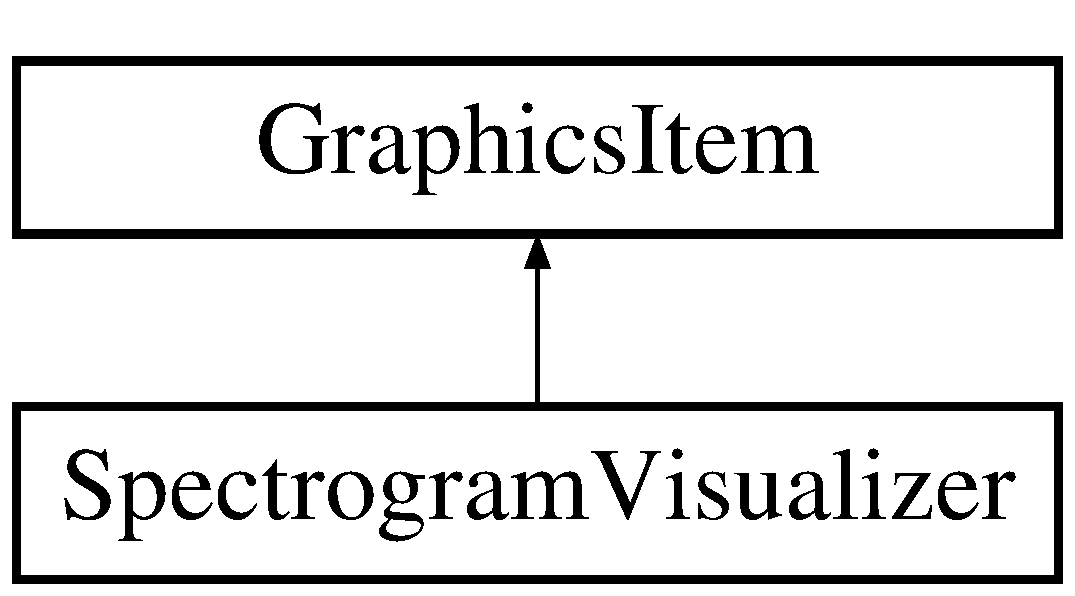
\includegraphics[height=2.000000cm]{classGraphicsItem}
\end{center}
\end{figure}
\subsection*{Public Member Functions}
\begin{DoxyCompactItemize}
\item 
\hypertarget{classGraphicsItem_a297b8c4f6ee3d69523af5593d73264d4}{}\label{classGraphicsItem_a297b8c4f6ee3d69523af5593d73264d4} 
virtual void {\bfseries display} ()=0
\item 
\hypertarget{classGraphicsItem_ae452e1227c8a9ebcc44318a0966f38c9}{}\label{classGraphicsItem_ae452e1227c8a9ebcc44318a0966f38c9} 
virtual void {\bfseries display\+Text} ()=0
\item 
\hypertarget{classGraphicsItem_a91cd9e4283de204b004501482f5b6fc1}{}\label{classGraphicsItem_a91cd9e4283de204b004501482f5b6fc1} 
virtual void {\bfseries idle} ()=0
\item 
\hypertarget{classGraphicsItem_a01cc49913f553f0defe6817e124b3314}{}\label{classGraphicsItem_a01cc49913f553f0defe6817e124b3314} 
virtual void {\bfseries pause} ()=0
\item 
\hypertarget{classGraphicsItem_a8591c77fe00af4be64101d3533f1d9d7}{}\label{classGraphicsItem_a8591c77fe00af4be64101d3533f1d9d7} 
virtual void {\bfseries keyboard} (unsigned char, int, int)=0
\item 
\hypertarget{classGraphicsItem_abd982a2447785360e944f7a92db27a14}{}\label{classGraphicsItem_abd982a2447785360e944f7a92db27a14} 
virtual void {\bfseries special} (int, int, int)=0
\item 
\hypertarget{classGraphicsItem_a7c5b5fc7929ffad1514be846ae1737f1}{}\label{classGraphicsItem_a7c5b5fc7929ffad1514be846ae1737f1} 
virtual void {\bfseries reshape} (int, int)=0
\item 
\hypertarget{classGraphicsItem_ae55ed569dcaf7749ce160436626fb0c0}{}\label{classGraphicsItem_ae55ed569dcaf7749ce160436626fb0c0} 
virtual void {\bfseries mouse} (int, int, int, int)=0
\item 
\hypertarget{classGraphicsItem_a6351546854c4b6e37d389b37da8fce2d}{}\label{classGraphicsItem_a6351546854c4b6e37d389b37da8fce2d} 
virtual void {\bfseries motion} (int, int)=0
\end{DoxyCompactItemize}
\subsection*{Protected Attributes}
\begin{DoxyCompactItemize}
\item 
\hypertarget{classGraphicsItem_a1a81e11e28f3ea510cd96c1eede3d905}{}\label{classGraphicsItem_a1a81e11e28f3ea510cd96c1eede3d905} 
bool {\bfseries is\+Paused}
\end{DoxyCompactItemize}


The documentation for this class was generated from the following file\+:\begin{DoxyCompactItemize}
\item 
Graphics\+Item.\+hpp\end{DoxyCompactItemize}

\hypertarget{classLog}{}\section{Log Class Reference}
\label{classLog}\index{Log@{Log}}


{\ttfamily \#include $<$Log.\+hpp$>$}

\subsection*{Public Member Functions}
\begin{DoxyCompactItemize}
\item 
\hyperlink{classLog_a0fbfda88fbee5027c89f6eb121059360}{$\sim$\+Log} ()
\item 
void \hyperlink{classLog_ac4365b77dc0b64c77e577888dfab5099}{log} (std\+::string \&message)
\item 
void \hyperlink{classLog_a60929e600b7759e97ea623ea5b05971e}{log} (const char $\ast$const message)
\item 
std\+::ostream \& \hyperlink{classLog_a32d048a4924c7851c4b7b16758675af6}{logger} ()
\end{DoxyCompactItemize}
\subsection*{Static Public Member Functions}
\begin{DoxyCompactItemize}
\item 
static \hyperlink{classLog}{Log} $\ast$ \hyperlink{classLog_a987f3ff401eea783d0e80daaea1d7aca}{get\+Instance} ()
\end{DoxyCompactItemize}


\subsection{Detailed Description}
Singleton class to handle logging to standard output or a file. 

\subsection{Constructor \& Destructor Documentation}
\hypertarget{classLog_a0fbfda88fbee5027c89f6eb121059360}{}\label{classLog_a0fbfda88fbee5027c89f6eb121059360} 
\index{Log@{Log}!````~Log@{$\sim$\+Log}}
\index{````~Log@{$\sim$\+Log}!Log@{Log}}
\subsubsection{\texorpdfstring{$\sim$\+Log()}{~Log()}}
{\ttfamily Log\+::$\sim$\+Log (\begin{DoxyParamCaption}{ }\end{DoxyParamCaption})}

De-\/allocates all dynamic memory. 

\subsection{Member Function Documentation}
\hypertarget{classLog_a987f3ff401eea783d0e80daaea1d7aca}{}\label{classLog_a987f3ff401eea783d0e80daaea1d7aca} 
\index{Log@{Log}!get\+Instance@{get\+Instance}}
\index{get\+Instance@{get\+Instance}!Log@{Log}}
\subsubsection{\texorpdfstring{get\+Instance()}{getInstance()}}
{\ttfamily \hyperlink{classLog}{Log} $\ast$ Log\+::get\+Instance (\begin{DoxyParamCaption}{ }\end{DoxyParamCaption})\hspace{0.3cm}{\ttfamily [static]}}

Accessor method for the singleton instance of the class. If the instance does not exist, then (and only then) a new instance is created. \begin{DoxyReturn}{Returns}

\end{DoxyReturn}
\hypertarget{classLog_ac4365b77dc0b64c77e577888dfab5099}{}\label{classLog_ac4365b77dc0b64c77e577888dfab5099} 
\index{Log@{Log}!log@{log}}
\index{log@{log}!Log@{Log}}
\subsubsection{\texorpdfstring{log()}{log()}\hspace{0.1cm}{\footnotesize\ttfamily [1/2]}}
{\ttfamily void Log\+::log (\begin{DoxyParamCaption}\item[{std\+::string \&}]{message }\end{DoxyParamCaption})}

Logging method for a string input. 
\begin{DoxyParams}{Parameters}
{\em message} & the message to log. \\
\hline
\end{DoxyParams}
\hypertarget{classLog_a60929e600b7759e97ea623ea5b05971e}{}\label{classLog_a60929e600b7759e97ea623ea5b05971e} 
\index{Log@{Log}!log@{log}}
\index{log@{log}!Log@{Log}}
\subsubsection{\texorpdfstring{log()}{log()}\hspace{0.1cm}{\footnotesize\ttfamily [2/2]}}
{\ttfamily void Log\+::log (\begin{DoxyParamCaption}\item[{const char $\ast$const}]{message }\end{DoxyParamCaption})}

Logging method for a const char$\ast$ const input. 
\begin{DoxyParams}{Parameters}
{\em message} & the message to log. \\
\hline
\end{DoxyParams}
\hypertarget{classLog_a32d048a4924c7851c4b7b16758675af6}{}\label{classLog_a32d048a4924c7851c4b7b16758675af6} 
\index{Log@{Log}!logger@{logger}}
\index{logger@{logger}!Log@{Log}}
\subsubsection{\texorpdfstring{logger()}{logger()}}
{\ttfamily std\+::ostream \& Log\+::logger (\begin{DoxyParamCaption}{ }\end{DoxyParamCaption})}

Returns the appropriate logger, according to Log\+::\+O\+U\+T\+P\+U\+T\+\_\+\+D\+I\+R\+E\+C\+T\+I\+ON. This is useful with the stream operator. \begin{DoxyReturn}{Returns}
appropriate logger, according to Log\+::\+O\+U\+T\+P\+U\+T\+\_\+\+D\+I\+R\+E\+C\+T\+I\+ON. See its documentation for more details. 
\end{DoxyReturn}


The documentation for this class was generated from the following files\+:\begin{DoxyCompactItemize}
\item 
Log.\+hpp\item 
Log.\+cpp\end{DoxyCompactItemize}

\hypertarget{classPortAudio}{}\section{Port\+Audio Class Reference}
\label{classPortAudio}\index{Port\+Audio@{Port\+Audio}}
Inheritance diagram for Port\+Audio\+:\begin{figure}[H]
\begin{center}
\leavevmode
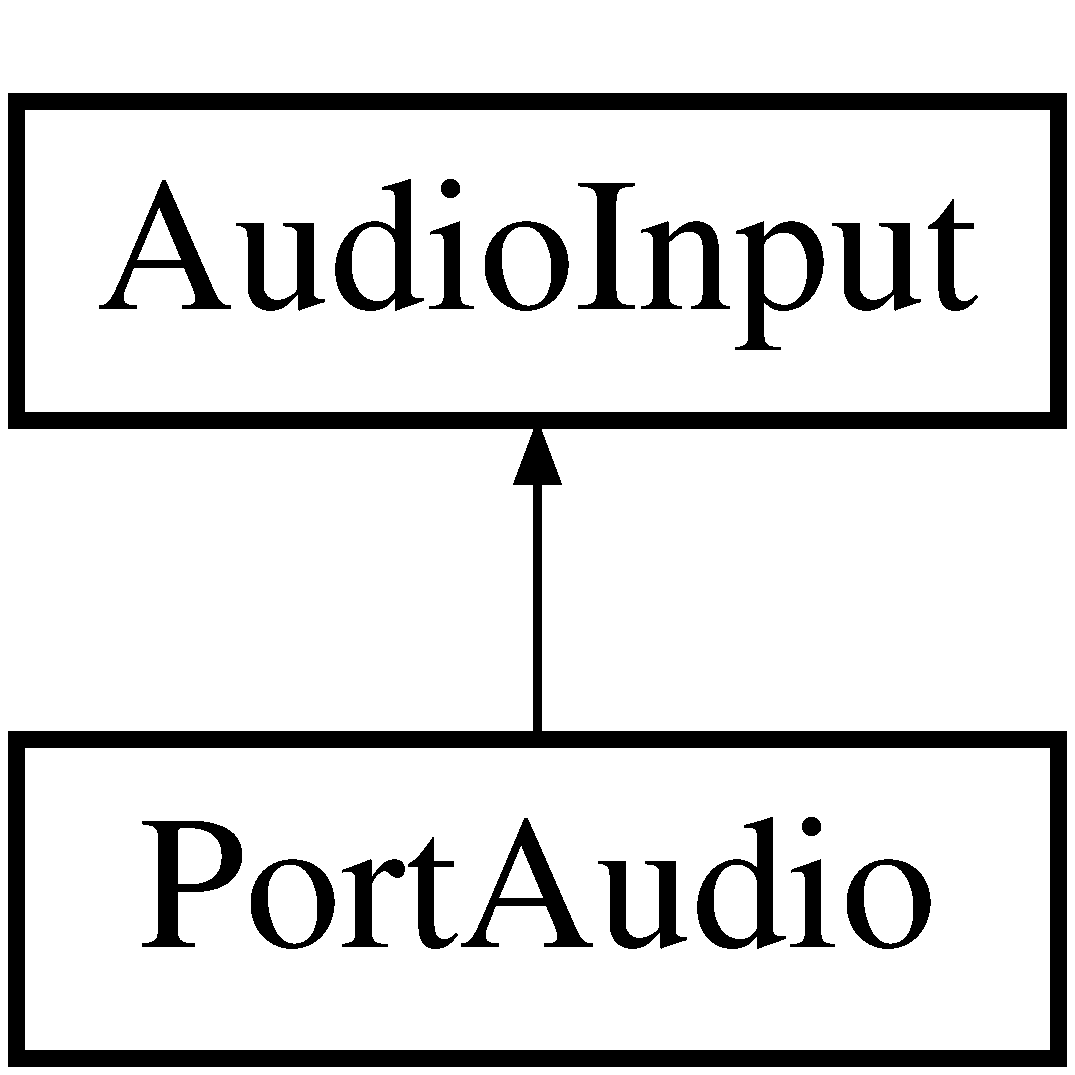
\includegraphics[height=2.000000cm]{classPortAudio}
\end{center}
\end{figure}
\subsection*{Public Member Functions}
\begin{DoxyCompactItemize}
\item 
\mbox{\hyperlink{classPortAudio_ae2b322ab89b7412a1bc61a4b02a20bf0}{Port\+Audio}} (int)
\item 
\mbox{\hyperlink{classPortAudio_a5f84a7247f216657c54993180fc18c6c}{Port\+Audio}} (const \mbox{\hyperlink{classPortAudio}{Port\+Audio}} \&)
\item 
\mbox{\Hypertarget{classPortAudio_aacb93627b1b3aa427cd3f357b7e20eb7}\label{classPortAudio_aacb93627b1b3aa427cd3f357b7e20eb7}} 
\mbox{\hyperlink{classPortAudio}{Port\+Audio}} \& {\bfseries operator=} (const \mbox{\hyperlink{classPortAudio}{Port\+Audio}} \&)
\item 
\mbox{\hyperlink{classPortAudio_a5f80fdff2377981fcd42fae42d4b65c3}{$\sim$\+Port\+Audio}} ()
\item 
int \mbox{\hyperlink{classPortAudio_a2685650c8e1568f8089babd3af5f6bc1}{start\+Capture}} ()
\item 
virtual void \mbox{\hyperlink{classPortAudio_a88fc85aad0b14014b0775ec0a769ea0a}{quit\+Now}} ()
\end{DoxyCompactItemize}
\subsection*{Static Public Member Functions}
\begin{DoxyCompactItemize}
\item 
static int \mbox{\hyperlink{classPortAudio_a006e388f2b3e886377390e1a97580d53}{audio\+In}} (const void $\ast$input\+Buffer, void $\ast$output\+Buffer, unsigned long num\+Samples, const Pa\+Stream\+Callback\+Time\+Info $\ast$time\+Info, Pa\+Stream\+Callback\+Flags status\+Flags, void $\ast$user\+Data)
\end{DoxyCompactItemize}
\subsection*{Additional Inherited Members}


\subsection{Detailed Description}


Definition at line 18 of file Port\+Audio.\+hpp.



\subsection{Constructor \& Destructor Documentation}
\mbox{\Hypertarget{classPortAudio_ae2b322ab89b7412a1bc61a4b02a20bf0}\label{classPortAudio_ae2b322ab89b7412a1bc61a4b02a20bf0}} 
\index{Port\+Audio@{Port\+Audio}!Port\+Audio@{Port\+Audio}}
\index{Port\+Audio@{Port\+Audio}!Port\+Audio@{Port\+Audio}}
\subsubsection{\texorpdfstring{Port\+Audio()}{PortAudio()}\hspace{0.1cm}{\footnotesize\ttfamily [1/2]}}
{\footnotesize\ttfamily Port\+Audio\+::\+Port\+Audio (\begin{DoxyParamCaption}\item[{int}]{requested\+Input\+Device\+Id }\end{DoxyParamCaption})}

Constructor 

Definition at line 8 of file Port\+Audio.\+cpp.


\begin{DoxyCode}
9   : \mbox{\hyperlink{classAudioInput_a51903411fbfb29b77f30a0ee3fbaa50e}{AudioInput}}()
10 \{
11     this->requestedInputDeviceId = requestedInputDeviceId;
12     \mbox{\hyperlink{classAudioInput_acfe371c4f5790bd67d282bc83225728e}{samplingRate}} = 44100;
13     \mbox{\hyperlink{classAudioInput_a8b6ea4cd6b88e5cd9d051b298efbb65e}{samplingPeriod}} = 1.0f/\mbox{\hyperlink{classAudioInput_acfe371c4f5790bd67d282bc83225728e}{samplingRate}};
14     \textcolor{comment}{//stream = nullptr;}
15     \mbox{\hyperlink{classAudioInput_aea3145ccca0f7cebf36a78278ca44031}{bufferMemorySeconds}} = 5;
16     \mbox{\hyperlink{classAudioInput_a4e213a9a22a62dccc3a54369101559c7}{bufferSizeSamples}} = \mbox{\hyperlink{classAudioInput_aea3145ccca0f7cebf36a78278ca44031}{bufferMemorySeconds}} * 
      \mbox{\hyperlink{classAudioInput_acfe371c4f5790bd67d282bc83225728e}{samplingRate}};
17     
18     \mbox{\hyperlink{classLog_a987f3ff401eea783d0e80daaea1d7aca}{Log::getInstance}}()->\mbox{\hyperlink{classLog_a32d048a4924c7851c4b7b16758675af6}{logger}}() << \textcolor{stringliteral}{"Buffer Size: "} << 
      \mbox{\hyperlink{classAudioInput_a4e213a9a22a62dccc3a54369101559c7}{bufferSizeSamples}} << \textcolor{stringliteral}{" samples."} << std::endl;
19     
20     \textcolor{comment}{/* initialize the audio buffer */}
21     \mbox{\hyperlink{classAudioInput_a797943485896a381ea80947c8b6a8488}{audioBuffer}} = \textcolor{keyword}{new} \textcolor{keywordtype}{float}[\mbox{\hyperlink{classAudioInput_a4e213a9a22a62dccc3a54369101559c7}{bufferSizeSamples}}];
22     \textcolor{keywordflow}{for} (\textcolor{keywordtype}{int} i = 0; i < \mbox{\hyperlink{classAudioInput_a4e213a9a22a62dccc3a54369101559c7}{bufferSizeSamples}}; ++i)
23     \{
24         \mbox{\hyperlink{classAudioInput_a797943485896a381ea80947c8b6a8488}{audioBuffer}}[i] = 0.0f;
25     \}
26 \}
\end{DoxyCode}
\mbox{\Hypertarget{classPortAudio_a5f84a7247f216657c54993180fc18c6c}\label{classPortAudio_a5f84a7247f216657c54993180fc18c6c}} 
\index{Port\+Audio@{Port\+Audio}!Port\+Audio@{Port\+Audio}}
\index{Port\+Audio@{Port\+Audio}!Port\+Audio@{Port\+Audio}}
\subsubsection{\texorpdfstring{Port\+Audio()}{PortAudio()}\hspace{0.1cm}{\footnotesize\ttfamily [2/2]}}
{\footnotesize\ttfamily Port\+Audio\+::\+Port\+Audio (\begin{DoxyParamCaption}\item[{const \mbox{\hyperlink{classPortAudio}{Port\+Audio}} \&}]{other }\end{DoxyParamCaption})}

Cony constructor 

Definition at line 28 of file Port\+Audio.\+cpp.


\begin{DoxyCode}
28                                            \{
29     this->stream = other.stream;
30     this->requestedInputDeviceId = other.requestedInputDeviceId;
31 \}
\end{DoxyCode}
\mbox{\Hypertarget{classPortAudio_a5f80fdff2377981fcd42fae42d4b65c3}\label{classPortAudio_a5f80fdff2377981fcd42fae42d4b65c3}} 
\index{Port\+Audio@{Port\+Audio}!````~Port\+Audio@{$\sim$\+Port\+Audio}}
\index{````~Port\+Audio@{$\sim$\+Port\+Audio}!Port\+Audio@{Port\+Audio}}
\subsubsection{\texorpdfstring{$\sim$\+Port\+Audio()}{~PortAudio()}}
{\footnotesize\ttfamily Port\+Audio\+::$\sim$\+Port\+Audio (\begin{DoxyParamCaption}{ }\end{DoxyParamCaption})}

Closes the audio capture stream and de-\/allocates any dynamic memory. 

Definition at line 41 of file Port\+Audio.\+cpp.


\begin{DoxyCode}
41                       \{
42     \textcolor{comment}{//delete stream;}
43 \}
\end{DoxyCode}


\subsection{Member Function Documentation}
\mbox{\Hypertarget{classPortAudio_a006e388f2b3e886377390e1a97580d53}\label{classPortAudio_a006e388f2b3e886377390e1a97580d53}} 
\index{Port\+Audio@{Port\+Audio}!audio\+In@{audio\+In}}
\index{audio\+In@{audio\+In}!Port\+Audio@{Port\+Audio}}
\subsubsection{\texorpdfstring{audio\+In()}{audioIn()}}
{\footnotesize\ttfamily int Port\+Audio\+::audio\+In (\begin{DoxyParamCaption}\item[{const void $\ast$}]{input\+Buffer,  }\item[{void $\ast$}]{output\+Buffer,  }\item[{unsigned long}]{num\+Samples,  }\item[{const Pa\+Stream\+Callback\+Time\+Info $\ast$}]{time\+Info,  }\item[{Pa\+Stream\+Callback\+Flags}]{status\+Flags,  }\item[{void $\ast$}]{user\+Data }\end{DoxyParamCaption})\hspace{0.3cm}{\ttfamily [static]}}

Callable used by a thread to continuously populate audio\+Buffer from the audio stream. 

Definition at line 45 of file Port\+Audio.\+cpp.


\begin{DoxyCode}
48 \{
49     \textcolor{comment}{//Log::getInstance()->logger() << "audioIn()" << std::endl;}
50     \mbox{\hyperlink{classPortAudio}{PortAudio}} *instance = (\mbox{\hyperlink{classPortAudio}{PortAudio}}*)customData;
51     \textcolor{keyword}{const} SAMPLE *in = (SAMPLE*)inputBuffer;
52     \textcolor{keywordtype}{int} index;
53     
54     \textcolor{comment}{/* prevent unused variable warnings */}
55     (void) outputBuffer;
56     (void) timeInfo;
57     (void) statusFlags;
58     
59     \textcolor{keywordflow}{if} (inputBuffer == NULL)
60     \{
61         \textcolor{comment}{/* silence */}
62         \textcolor{keywordflow}{for} (\textcolor{keywordtype}{int} i = 0; i < numSamples; ++i)
63         \{
64             index = mod(instance->\mbox{\hyperlink{classAudioInput_a3c9888a90ca8bc6b42257f3f11ee9a6e}{bufferIndex}} + i, instance->
      \mbox{\hyperlink{classAudioInput_a4e213a9a22a62dccc3a54369101559c7}{bufferSizeSamples}});
65             instance->\mbox{\hyperlink{classAudioInput_a797943485896a381ea80947c8b6a8488}{audioBuffer}}[index] = SAMPLE\_SILENCE; \textcolor{comment}{/* left channel */}
66             \textcolor{comment}{//if (NUM\_CHANNELS == 2) audioBuffer[i] = SAMPLE\_SILENCE; /* right channel */}
67         \}
68     \}
69     \textcolor{keywordflow}{else}
70     \{
71         \textcolor{comment}{/* non-silence */}
72         \textcolor{comment}{//Log::getInstance()->logger() << in[numSamples - 1] << std::endl;}
73         \textcolor{keywordflow}{for} (\textcolor{keywordtype}{int} i = 0; i < numSamples; ++i)
74         \{
75             index = mod(instance->\mbox{\hyperlink{classAudioInput_a3c9888a90ca8bc6b42257f3f11ee9a6e}{bufferIndex}} + i, instance->
      \mbox{\hyperlink{classAudioInput_a4e213a9a22a62dccc3a54369101559c7}{bufferSizeSamples}});
76             instance->\mbox{\hyperlink{classAudioInput_a797943485896a381ea80947c8b6a8488}{audioBuffer}}[index] = in[i]; \textcolor{comment}{/* left channel */}
77             \textcolor{comment}{//if (NUM\_CHANNELS == 2) audioBuffer[i] = *in++; /* right channel */}
78         \}
79     \}
80     instance->\mbox{\hyperlink{classAudioInput_a3c9888a90ca8bc6b42257f3f11ee9a6e}{bufferIndex}} = mod(instance->\mbox{\hyperlink{classAudioInput_a3c9888a90ca8bc6b42257f3f11ee9a6e}{bufferIndex}} + numSamples, instance->
      \mbox{\hyperlink{classAudioInput_a4e213a9a22a62dccc3a54369101559c7}{bufferSizeSamples}});
81     \mbox{\hyperlink{classAudioInput_a77614769e39be88bbf5d78adf84d9260}{computeSpectrogramSlice}}(instance);
82     
83     \textcolor{comment}{//Log::getInstance()->logger() << "Buffer Index: " << instance->bufferIndex << std::endl;}
84     \textcolor{comment}{//Log::getInstance()->logger() << "# Samples: " << numSamples << ", Size: " <<
       instance->bufferSizeSamples << std::endl;}
85     
86     \textcolor{keywordflow}{return} instance->\mbox{\hyperlink{classAudioInput_aceef1c12e4f78624ed695371adf495df}{quit}} ? paComplete : paContinue;
87 \}
\end{DoxyCode}
\mbox{\Hypertarget{classPortAudio_a88fc85aad0b14014b0775ec0a769ea0a}\label{classPortAudio_a88fc85aad0b14014b0775ec0a769ea0a}} 
\index{Port\+Audio@{Port\+Audio}!quit\+Now@{quit\+Now}}
\index{quit\+Now@{quit\+Now}!Port\+Audio@{Port\+Audio}}
\subsubsection{\texorpdfstring{quit\+Now()}{quitNow()}}
{\footnotesize\ttfamily void Port\+Audio\+::quit\+Now (\begin{DoxyParamCaption}{ }\end{DoxyParamCaption})\hspace{0.3cm}{\ttfamily [virtual]}}

Defines how the instance stops the audio stream. 

Implements \mbox{\hyperlink{classAudioInput_a4fce5476455b1df813f1cb6eebb08311}{Audio\+Input}}.



Definition at line 89 of file Port\+Audio.\+cpp.


\begin{DoxyCode}
90 \{
91     \mbox{\hyperlink{classLog_a987f3ff401eea783d0e80daaea1d7aca}{Log::getInstance}}()->\mbox{\hyperlink{classLog_a32d048a4924c7851c4b7b16758675af6}{logger}}() << \textcolor{stringliteral}{"Quitting."} << std::endl;
92     \textcolor{comment}{/* raise the quit flag to signal to the audio capture thread to stop polling for audio */}
93     \mbox{\hyperlink{classAudioInput_aceef1c12e4f78624ed695371adf495df}{quit}} = \textcolor{keyword}{true};
94 
95     \textcolor{comment}{/* close the stream */}
96     \mbox{\hyperlink{classLog_a987f3ff401eea783d0e80daaea1d7aca}{Log::getInstance}}()->\mbox{\hyperlink{classLog_a32d048a4924c7851c4b7b16758675af6}{logger}}() << \textcolor{stringliteral}{"Closing stream."} << std::endl;
97     PaError err;
98     err = Pa\_CloseStream(stream);
99     \textcolor{keywordflow}{if} (err != paNoError) \{
100         \mbox{\hyperlink{classLog_a987f3ff401eea783d0e80daaea1d7aca}{Log::getInstance}}()->\mbox{\hyperlink{classLog_a32d048a4924c7851c4b7b16758675af6}{logger}}() << \textcolor{stringliteral}{"PortAudio stream close error: "} << 
      Pa\_GetErrorText(err) << std::endl;
101     \}
102     
103     \textcolor{comment}{/* terminate portaudio */}
104     \mbox{\hyperlink{classLog_a987f3ff401eea783d0e80daaea1d7aca}{Log::getInstance}}()->\mbox{\hyperlink{classLog_a32d048a4924c7851c4b7b16758675af6}{logger}}() << \textcolor{stringliteral}{"Terminating PortAudio."} << std::endl;
105     err = Pa\_Terminate();
106     \textcolor{keywordflow}{if} (err != paNoError) \{
107         \mbox{\hyperlink{classLog_a987f3ff401eea783d0e80daaea1d7aca}{Log::getInstance}}()->\mbox{\hyperlink{classLog_a32d048a4924c7851c4b7b16758675af6}{logger}}() << \textcolor{stringliteral}{"PortAudio termination error: "} << 
      Pa\_GetErrorText(err) << std::endl;
108     \}
109 \}
\end{DoxyCode}
\mbox{\Hypertarget{classPortAudio_a2685650c8e1568f8089babd3af5f6bc1}\label{classPortAudio_a2685650c8e1568f8089babd3af5f6bc1}} 
\index{Port\+Audio@{Port\+Audio}!start\+Capture@{start\+Capture}}
\index{start\+Capture@{start\+Capture}!Port\+Audio@{Port\+Audio}}
\subsubsection{\texorpdfstring{start\+Capture()}{startCapture()}}
{\footnotesize\ttfamily int Port\+Audio\+::start\+Capture (\begin{DoxyParamCaption}{ }\end{DoxyParamCaption})\hspace{0.3cm}{\ttfamily [virtual]}}

Begins capturing the audio stream. \begin{DoxyReturn}{Returns}
indication of capture success or failure. 0 -\/$>$ successfull setup. else -\/$>$ failed setup. 
\end{DoxyReturn}


Implements \mbox{\hyperlink{classAudioInput_afa753742035f7069f5ef0c2ece6a62fe}{Audio\+Input}}.



Definition at line 111 of file Port\+Audio.\+cpp.


\begin{DoxyCode}
112 \{
113     PaError err;
114     
115     err = Pa\_Initialize();
116     \textcolor{keywordflow}{if} (err != paNoError) \{
117         \mbox{\hyperlink{classLog_a987f3ff401eea783d0e80daaea1d7aca}{Log::getInstance}}()->\mbox{\hyperlink{classLog_a32d048a4924c7851c4b7b16758675af6}{logger}}() << \textcolor{stringliteral}{"PortAudio initialization error: "} << 
      Pa\_GetErrorText(err) << std::endl;
118         \textcolor{keywordflow}{return} 1;
119     \}
120 
121     \mbox{\hyperlink{classLog_a987f3ff401eea783d0e80daaea1d7aca}{Log::getInstance}}()->\mbox{\hyperlink{classLog_a32d048a4924c7851c4b7b16758675af6}{logger}}() << \textcolor{stringliteral}{"Opening input stream for device #"} << 
      requestedInputDeviceId << std::endl;
122 
123     \textcolor{comment}{/* initialize and populate desired input stream parameters */}
124     PaStreamParameters inputParams;
125     \textcolor{keyword}{const} PaDeviceInfo *deviceInfo;
126     memset(&inputParams, 0, \textcolor{keyword}{sizeof}(inputParams));
127     deviceInfo = Pa\_GetDeviceInfo(requestedInputDeviceId);
128     inputParams.channelCount = 1;\textcolor{comment}{//deviceInfo->maxInputChannels;}
129     inputParams.sampleFormat = paFloat32;
130     inputParams.suggestedLatency = deviceInfo->defaultLowInputLatency;
131     inputParams.hostApiSpecificStreamInfo = NULL;
132 
133     err = Pa\_OpenStream(
134             &stream,
135             &inputParams,
136             NULL,
137             44100,
138             paFramesPerBufferUnspecified,
139             paNoFlag,
140             \mbox{\hyperlink{classPortAudio_a006e388f2b3e886377390e1a97580d53}{audioIn}},
141             (\textcolor{keywordtype}{void}*)\textcolor{keyword}{this}
142     );
143     
144     \textcolor{comment}{/* TODO if opening the default stream fails, give the user device info */}
145     \textcolor{keywordflow}{if} (err != paNoError) \{
146         \mbox{\hyperlink{classLog_a987f3ff401eea783d0e80daaea1d7aca}{Log::getInstance}}()->\mbox{\hyperlink{classLog_a32d048a4924c7851c4b7b16758675af6}{logger}}() << \textcolor{stringliteral}{"PortAudio error opening default stream: "} <<
       Pa\_GetErrorText(err) << std::endl;
147 
148         \textcolor{comment}{/* TODO */}
149         \textcolor{keywordflow}{return} 1;
150     \}
151 
152     \textcolor{comment}{/* start the audio stream */}
153     err = Pa\_StartStream(stream);
154     \textcolor{keywordflow}{if} (err != paNoError) \{
155         \mbox{\hyperlink{classLog_a987f3ff401eea783d0e80daaea1d7aca}{Log::getInstance}}()->\mbox{\hyperlink{classLog_a32d048a4924c7851c4b7b16758675af6}{logger}}() << \textcolor{stringliteral}{"PortAudio starting stream: "} << 
      Pa\_GetErrorText(err) << std::endl;
156         \textcolor{keywordflow}{return} 1;
157     \}
158     
159     \mbox{\hyperlink{classLog_a987f3ff401eea783d0e80daaea1d7aca}{Log::getInstance}}()->\mbox{\hyperlink{classLog_a32d048a4924c7851c4b7b16758675af6}{logger}}() << \textcolor{stringliteral}{"Successfully starting sampling audio."} << 
      std::endl;
160     \textcolor{keywordflow}{return} 0;
161 \}
\end{DoxyCode}


The documentation for this class was generated from the following files\+:\begin{DoxyCompactItemize}
\item 
src/Port\+Audio.\+hpp\item 
src/Port\+Audio.\+cpp\end{DoxyCompactItemize}

\hypertarget{structSpectrogramVisualizer_1_1shortcuts}{}\section{Spectrogram\+Visualizer\+:\+:shortcuts Struct Reference}
\label{structSpectrogramVisualizer_1_1shortcuts}\index{Spectrogram\+Visualizer\+::shortcuts@{Spectrogram\+Visualizer\+::shortcuts}}


{\ttfamily \#include $<$Spectrogram\+Visualizer.\+hpp$>$}

\subsection*{Public Attributes}
\begin{DoxyCompactItemize}
\item 
\hypertarget{structSpectrogramVisualizer_1_1shortcuts_a3c916b79eb5fdbc9261962946104b26f}{}\label{structSpectrogramVisualizer_1_1shortcuts_a3c916b79eb5fdbc9261962946104b26f} 
char {\bfseries E\+S\+C\+A\+PE}
\item 
\hypertarget{structSpectrogramVisualizer_1_1shortcuts_a2ce860bc091bea9e78da24cd5691c4b4}{}\label{structSpectrogramVisualizer_1_1shortcuts_a2ce860bc091bea9e78da24cd5691c4b4} 
char {\bfseries Q\+U\+IT}
\item 
\hypertarget{structSpectrogramVisualizer_1_1shortcuts_a260568371342c5408ebb130ffa09cb33}{}\label{structSpectrogramVisualizer_1_1shortcuts_a260568371342c5408ebb130ffa09cb33} 
char {\bfseries D\+I\+A\+G\+N\+O\+SE}
\item 
\hypertarget{structSpectrogramVisualizer_1_1shortcuts_a0c36f6e4ee64ad69c86e75fb0c986c00}{}\label{structSpectrogramVisualizer_1_1shortcuts_a0c36f6e4ee64ad69c86e75fb0c986c00} 
char {\bfseries P\+A\+U\+SE}
\item 
\hypertarget{structSpectrogramVisualizer_1_1shortcuts_a19b5a234ecbb017c1dbcff99775f850a}{}\label{structSpectrogramVisualizer_1_1shortcuts_a19b5a234ecbb017c1dbcff99775f850a} 
char {\bfseries S\+A\+M\+P\+L\+E\+\_\+\+R\+A\+T\+E\+\_\+\+UP}
\item 
\hypertarget{structSpectrogramVisualizer_1_1shortcuts_addbcd297e9bd96d574b8d0f04c363c9c}{}\label{structSpectrogramVisualizer_1_1shortcuts_addbcd297e9bd96d574b8d0f04c363c9c} 
char {\bfseries S\+A\+M\+P\+L\+E\+\_\+\+R\+A\+T\+E\+\_\+\+D\+O\+WN}
\item 
\hypertarget{structSpectrogramVisualizer_1_1shortcuts_ab233bdefbc2be60b645f8096c36a6966}{}\label{structSpectrogramVisualizer_1_1shortcuts_ab233bdefbc2be60b645f8096c36a6966} 
char {\bfseries C\+H\+A\+N\+G\+E\+\_\+\+C\+O\+L\+O\+R\+\_\+\+S\+C\+H\+E\+ME}
\end{DoxyCompactItemize}


\subsection{Detailed Description}
Struct with multiple char\textquotesingle{}s representing specific keyboard keys corresponding to desired program actions. 

The documentation for this struct was generated from the following file\+:\begin{DoxyCompactItemize}
\item 
Spectrogram\+Visualizer.\+hpp\end{DoxyCompactItemize}

\hypertarget{structSpectrogramVisualizer}{}\section{Spectrogram\+Visualizer Class Reference}
\label{structSpectrogramVisualizer}\index{Spectrogram\+Visualizer@{Spectrogram\+Visualizer}}


{\ttfamily \#include $<$Spectrogram\+Visualizer.\+hpp$>$}

Inheritance diagram for Spectrogram\+Visualizer\+:\begin{figure}[H]
\begin{center}
\leavevmode
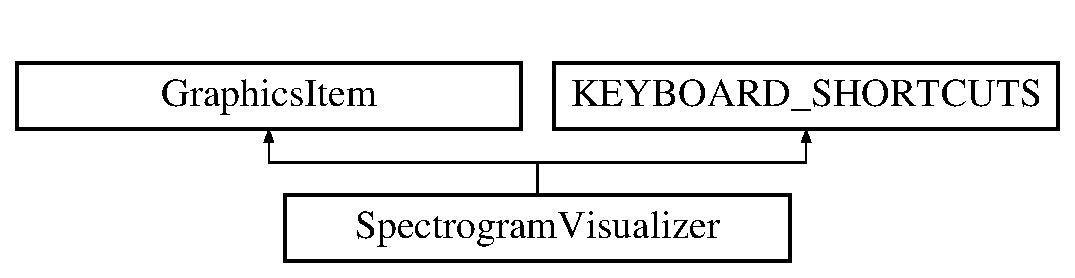
\includegraphics[height=2.000000cm]{structSpectrogramVisualizer}
\end{center}
\end{figure}
\subsection*{Classes}
\begin{DoxyCompactItemize}
\item 
struct \mbox{\hyperlink{structSpectrogramVisualizer_1_1shortcuts}{shortcuts}}
\end{DoxyCompactItemize}
\subsection*{Public Member Functions}
\begin{DoxyCompactItemize}
\item 
\mbox{\hyperlink{structSpectrogramVisualizer_a7b971af130bf95c4f307e2add2468825}{Spectrogram\+Visualizer}} (int, int)
\item 
\mbox{\Hypertarget{structSpectrogramVisualizer_a483fbc5948a64946b397ebb6d54146b6}\label{structSpectrogramVisualizer_a483fbc5948a64946b397ebb6d54146b6}} 
{\bfseries Spectrogram\+Visualizer} (const \mbox{\hyperlink{structSpectrogramVisualizer}{Spectrogram\+Visualizer}} \&)
\item 
\mbox{\Hypertarget{structSpectrogramVisualizer_a2212e878cb2cf147fd885989e511ed77}\label{structSpectrogramVisualizer_a2212e878cb2cf147fd885989e511ed77}} 
\mbox{\hyperlink{structSpectrogramVisualizer}{Spectrogram\+Visualizer}} \& {\bfseries operator=} (const \mbox{\hyperlink{structSpectrogramVisualizer}{Spectrogram\+Visualizer}} \&)
\item 
\mbox{\hyperlink{structSpectrogramVisualizer_a2b55364382a4ee290918a05946505561}{$\sim$\+Spectrogram\+Visualizer}} ()
\item 
virtual void \mbox{\hyperlink{structSpectrogramVisualizer_a529c64c733ffc564764593329c483ae2}{display}} ()
\item 
virtual void \mbox{\hyperlink{structSpectrogramVisualizer_a9b9aa780d95f710b1c876ce49abac9a1}{display\+Text}} ()
\item 
virtual void \mbox{\hyperlink{structSpectrogramVisualizer_a669c19fe9dc24dc89e1cc518edb24de6}{idle}} ()
\item 
virtual void \mbox{\hyperlink{structSpectrogramVisualizer_a301989369e63d88cd6a59d12c23b4551}{pause}} ()
\item 
virtual void \mbox{\hyperlink{structSpectrogramVisualizer_a2901f4ea1e35d4c7e6660f6c19ed468f}{keyboard}} (unsigned char key, int x\+Pos, int y\+Pos)
\item 
virtual void \mbox{\hyperlink{structSpectrogramVisualizer_a631d3522ef8d8bdc6fd9ba9acf2f15ec}{special}} (int key, int x\+Pos, int y\+Pos)
\item 
virtual void \mbox{\hyperlink{structSpectrogramVisualizer_a789c6b59ab3a6960056eaab014163b91}{reshape}} (int w, int h)
\item 
virtual void \mbox{\hyperlink{structSpectrogramVisualizer_a949b2e0bfd260e6f8d63b5867f1b4edf}{mouse}} (int button, int state, int x, int y)
\item 
virtual void \mbox{\hyperlink{structSpectrogramVisualizer_a8ab333867c86cfa188ff026410e271aa}{motion}} (int x, int y)
\end{DoxyCompactItemize}
\subsection*{Public Attributes}
\begin{DoxyCompactItemize}
\item 
\mbox{\Hypertarget{structSpectrogramVisualizer_add6b6c6e7a1768bd6fef3256f1cb26bc}\label{structSpectrogramVisualizer_add6b6c6e7a1768bd6fef3256f1cb26bc}} 
{\bfseries q}
\item 
\mbox{\Hypertarget{structSpectrogramVisualizer_a969c09495e18bec03ba7145b967b6cf7}\label{structSpectrogramVisualizer_a969c09495e18bec03ba7145b967b6cf7}} 
{\bfseries d}
\end{DoxyCompactItemize}
\subsection*{Static Public Attributes}
\begin{DoxyCompactItemize}
\item 
static const char $\ast$const \mbox{\hyperlink{structSpectrogramVisualizer_ad833647df19d8ae0eb2e47efe989d1d9}{note\+Names}} \mbox{[}$\,$\mbox{]}
\item 
static const \mbox{\hyperlink{structSpectrogramVisualizer_1_1shortcuts}{shortcuts}} \mbox{\hyperlink{structSpectrogramVisualizer_a20eb03afddbbde072d82b1efe675b0f3}{K\+E\+Y\+B\+O\+A\+R\+D\+\_\+\+S\+H\+O\+R\+T\+C\+U\+TS}}
\item 
static const float \mbox{\hyperlink{structSpectrogramVisualizer_adfe2ed143313d59d7c118cadec1460b9}{M\+I\+D\+D\+L\+E\+\_\+\+C\+\_\+\+F\+R\+E\+Q\+U\+E\+N\+CY}} = 261.\+626f
\item 
static const unsigned int \mbox{\hyperlink{structSpectrogramVisualizer_affbdeff0d7b800feb17aab0a367222da}{N\+\_\+\+S\+E\+M\+I\+T\+O\+N\+E\+S\+\_\+\+P\+E\+R\+\_\+\+O\+C\+T\+A\+VE}} = 12
\end{DoxyCompactItemize}
\subsection*{Additional Inherited Members}


\subsection{Detailed Description}
Obtains and draws a spectrogram from continuous audio input. Implements methods from the abstract class \mbox{\hyperlink{classGraphicsItem}{Graphics\+Item}}, which are called by a subject \mbox{\hyperlink{classDisplay}{Display}} instance as an implementation of the observer design pattern. \begin{DoxyAuthor}{Author}
Anthony Agnone, Aug 2016 
\end{DoxyAuthor}


Definition at line 9 of file Spectrogram\+Visualizer.\+cpp.



\subsection{Constructor \& Destructor Documentation}
\mbox{\Hypertarget{structSpectrogramVisualizer_a7b971af130bf95c4f307e2add2468825}\label{structSpectrogramVisualizer_a7b971af130bf95c4f307e2add2468825}} 
\index{Spectrogram\+Visualizer@{Spectrogram\+Visualizer}!Spectrogram\+Visualizer@{Spectrogram\+Visualizer}}
\index{Spectrogram\+Visualizer@{Spectrogram\+Visualizer}!Spectrogram\+Visualizer@{Spectrogram\+Visualizer}}
\subsubsection{\texorpdfstring{Spectrogram\+Visualizer()}{SpectrogramVisualizer()}}
{\footnotesize\ttfamily Spectrogram\+Visualizer\+::\+Spectrogram\+Visualizer (\begin{DoxyParamCaption}\item[{int}]{scroll\+Factor,  }\item[{int}]{requested\+Input\+Device\+Id }\end{DoxyParamCaption})}

Overloaded constructor to initialize various member parameters. 

Definition at line 21 of file Spectrogram\+Visualizer.\+cpp.


\begin{DoxyCode}
21                                                                                          \{
22     isPaused = \textcolor{keyword}{false};
23     colorScale[0] = 100.0f;     \textcolor{comment}{// 8-bit intensity offset}
24     colorScale[1] = 255 / 120.0f;     \textcolor{comment}{// 8-bit intensity slope (per dB units)}
25     audioInput = \textcolor{keyword}{new} \mbox{\hyperlink{classPortAudio}{PortAudio}}(requestedInputDeviceId);
26     \textcolor{keywordtype}{unsigned} \textcolor{keywordtype}{int} spectrogramSize = audioInput->getSpectrogramSize();
27 
28     spectrogramBytes = \textcolor{keyword}{new} \textcolor{keywordtype}{char}[spectrogramSize];
29     zeros(spectrogramBytes, spectrogramSize);
30 
31     spectrogramFloat = \textcolor{keyword}{new} \textcolor{keywordtype}{float}[spectrogramSize];
32     zeros(spectrogramFloat, spectrogramSize);
33 
34     highestFrequency = audioInput->getSamplingRate() / 2.0f;
35     hzPerPixelY = (float) highestFrequency / viewportSize[1];
36     hzPerPixelX = (float) highestFrequency / viewportSize[0];
37     fpsTick = time(\textcolor{keyword}{nullptr});
38     frameCount = 0;
39     fps = 0;
40     colorMode = 2;
41     this->scrollFactor = scrollFactor;
42     scrollCount = 0;
43     gettimeofday(&startTime, \textcolor{keyword}{nullptr});
44     runTime = 0.0;
45     frequencyReadOff = 0;
46     diagnose = \textcolor{keyword}{false};
47     strcpy(diagnosis, \textcolor{stringliteral}{"no diagnosis ..."});
48 
49     OUT(\textcolor{stringliteral}{"Highest Frequency: "} << highestFrequency);
50 
51     specId = 7;
52 \textcolor{preprocessor}{#ifdef DISPLAY\_SPECTROGRAM}
53     glGenTextures(14, &specId);
54     glBindTexture(GL\_TEXTURE\_2D, specId);
55     glTexParameteri(GL\_TEXTURE\_2D, GL\_TEXTURE\_WRAP\_S, GL\_REPEAT);
56     glTexParameteri(GL\_TEXTURE\_2D, GL\_TEXTURE\_WRAP\_T, GL\_REPEAT);
57     glTexParameteri(GL\_TEXTURE\_2D, GL\_TEXTURE\_MIN\_FILTER, GL\_LINEAR);
58     glTexParameteri(GL\_TEXTURE\_2D, GL\_TEXTURE\_MAG\_FILTER, GL\_LINEAR);
59 \textcolor{preprocessor}{#endif}
60 
61     \textcolor{comment}{/* notify the AudioInput instance that it should start capturing audio */}
62     \textcolor{keywordflow}{if}(audioInput->\mbox{\hyperlink{classAudioInput_afa753742035f7069f5ef0c2ece6a62fe}{startCapture}}() != 0) \{
63         OUT(\textcolor{stringliteral}{"Failed to start capturing audio."});
64         \textcolor{keywordflow}{throw} 99;
65     \}
66 \}
\end{DoxyCode}
\mbox{\Hypertarget{structSpectrogramVisualizer_a2b55364382a4ee290918a05946505561}\label{structSpectrogramVisualizer_a2b55364382a4ee290918a05946505561}} 
\index{Spectrogram\+Visualizer@{Spectrogram\+Visualizer}!````~Spectrogram\+Visualizer@{$\sim$\+Spectrogram\+Visualizer}}
\index{````~Spectrogram\+Visualizer@{$\sim$\+Spectrogram\+Visualizer}!Spectrogram\+Visualizer@{Spectrogram\+Visualizer}}
\subsubsection{\texorpdfstring{$\sim$\+Spectrogram\+Visualizer()}{~SpectrogramVisualizer()}}
{\footnotesize\ttfamily Spectrogram\+Visualizer\+::$\sim$\+Spectrogram\+Visualizer (\begin{DoxyParamCaption}{ }\end{DoxyParamCaption})}

Empty destructor. 

Definition at line 124 of file Spectrogram\+Visualizer.\+cpp.


\begin{DoxyCode}
124                                               \{
125     \textcolor{comment}{// this causes a seg fault?}
126     \textcolor{comment}{//if (audioInput != nullptr) delete audioInput;}
127 
128     \textcolor{keyword}{delete}[] spectrogramBytes;
129     \textcolor{keyword}{delete}[] spectrogramFloat;
130 \}
\end{DoxyCode}


\subsection{Member Function Documentation}
\mbox{\Hypertarget{structSpectrogramVisualizer_a529c64c733ffc564764593329c483ae2}\label{structSpectrogramVisualizer_a529c64c733ffc564764593329c483ae2}} 
\index{Spectrogram\+Visualizer@{Spectrogram\+Visualizer}!display@{display}}
\index{display@{display}!Spectrogram\+Visualizer@{Spectrogram\+Visualizer}}
\subsubsection{\texorpdfstring{display()}{display()}}
{\footnotesize\ttfamily void Spectrogram\+Visualizer\+::display (\begin{DoxyParamCaption}{ }\end{DoxyParamCaption})\hspace{0.3cm}{\ttfamily [virtual]}}

Displays all information and graphics on the screen. This function is routinely called by the \mbox{\hyperlink{classDisplay}{Display}} subject, and is one of many functions that the class defines as a \mbox{\hyperlink{classGraphicsItem}{Graphics\+Item}} observer in the observer design pattern. 

Implements \mbox{\hyperlink{classGraphicsItem}{Graphics\+Item}}.



Definition at line 464 of file Spectrogram\+Visualizer.\+cpp.


\begin{DoxyCode}
464                                     \{
465 \textcolor{preprocessor}{#ifdef DEBUG}
466     \textcolor{comment}{/* for sanity checking, draw boundary lines for the plot area in green */}
467     glMatrixMode(GL\_MODELVIEW);
468     glPushMatrix(); \textcolor{comment}{// use modelview matrix to transform [-lookbackSeconds,0]x[-1,1] somewhere}
469     glTranslatef(0.001, 0.001, 0);   \textcolor{comment}{// decide the location of 0,0 of the plot}
470     glScalef(0.999, 0.995, 1.0);  \textcolor{comment}{// x-scale for freq-units, y-scale for dB}
471     glColor4f(0.0, 1.0, 0.0, 1);
472     \textcolor{keywordtype}{int} xStart = 0.0, xEnd = 1.0;
473     \textcolor{keywordtype}{int} yStart = 0.0, yEnd = 1.0;
474     glBegin(GL\_LINE\_LOOP);
475         glVertex2f(xStart, yStart);
476         glVertex2f(xEnd, yStart);
477         glVertex2f(xEnd, yEnd);
478         glVertex2f(xStart, yEnd);
479         glVertex2f(xStart, yStart);
480     glEnd();
481     glPopMatrix();
482     glColor4f(0.7, 1.0, 1.0, 1);
483 \textcolor{preprocessor}{#endif}
484 
485 \textcolor{preprocessor}{#ifdef DISPLAY\_TIME}
486     plotTimeDomain();
487 \textcolor{preprocessor}{#endif}
488 
489 \textcolor{preprocessor}{#ifdef DISPLAY\_SPECMAG}
490     plotSpectralMagnitude();
491 \textcolor{preprocessor}{#endif}
492 
493 \textcolor{preprocessor}{#ifdef DISPLAY\_SPECTROGRAM}
494     plotSpectrogram();
495     scrollSpectrogram();
496     ++scrollCount;
497     \textcolor{keywordflow}{if} (scrollCount == SpectrogramVisualizer::scrollFactor) \{
498         scrollCount = 0;
499     \}
500 \textcolor{preprocessor}{#endif}
501 
502 \textcolor{preprocessor}{#ifdef DISPLAY\_TEXT}
503     \mbox{\hyperlink{structSpectrogramVisualizer_a9b9aa780d95f710b1c876ce49abac9a1}{displayText}}();
504 \textcolor{preprocessor}{#endif}
505 
506 \}
\end{DoxyCode}
\mbox{\Hypertarget{structSpectrogramVisualizer_a9b9aa780d95f710b1c876ce49abac9a1}\label{structSpectrogramVisualizer_a9b9aa780d95f710b1c876ce49abac9a1}} 
\index{Spectrogram\+Visualizer@{Spectrogram\+Visualizer}!display\+Text@{display\+Text}}
\index{display\+Text@{display\+Text}!Spectrogram\+Visualizer@{Spectrogram\+Visualizer}}
\subsubsection{\texorpdfstring{display\+Text()}{displayText()}}
{\footnotesize\ttfamily void Spectrogram\+Visualizer\+::display\+Text (\begin{DoxyParamCaption}{ }\end{DoxyParamCaption})\hspace{0.3cm}{\ttfamily [virtual]}}

Displays all text on the canvas. 

Implements \mbox{\hyperlink{classGraphicsItem}{Graphics\+Item}}.



Definition at line 508 of file Spectrogram\+Visualizer.\+cpp.


\begin{DoxyCode}
508                                         \{
509     glEnable(GL\_BLEND); \textcolor{comment}{// glBlendFunc (GL\_ONE,GL\_ZERO); // overwrite entirely}
510     glBlendFunc(GL\_ONE, GL\_ONE\_MINUS\_SRC\_ALPHA);
511 
512     glColor4f(1, .4, .4, 1.0); \textcolor{comment}{// write FPS, other params... coords in unit square}
513     \textcolor{keywordtype}{char} str[50];
514     sprintf(str, \textcolor{stringliteral}{"%d FPS"}, fps);
515     \mbox{\hyperlink{classDisplay_ac62e7e33c27d8c012c3efb8c07f3fc11}{Display::smallText}}(0.92, 0.96, str);
516     sprintf(str, \textcolor{stringliteral}{"gain offset %.0f dB"}, colorScale[0]);
517     \mbox{\hyperlink{classDisplay_ac62e7e33c27d8c012c3efb8c07f3fc11}{Display::smallText}}(0.02, 0.04, str);
518     sprintf(str, \textcolor{stringliteral}{"dyn range  %.1f dB"}, 255.0 / colorScale[1]);
519     \mbox{\hyperlink{classDisplay_ac62e7e33c27d8c012c3efb8c07f3fc11}{Display::smallText}}(0.02, 0.02, str);
520 
521     \textcolor{keywordflow}{if} (diagnose) \{  \textcolor{comment}{// show diagnosis}
522         glColor4f(.2, .2, .2, 0.8);  \textcolor{comment}{// transparent box}
523         glMatrixMode(GL\_MODELVIEW);
524         glPushMatrix(); \textcolor{comment}{// use modelview matrix to transform unit square to text box}
525         glTranslatef(0.5, 0.5, 0);
526         glScalef(0.5, 0.4, 1);
527         glTranslatef(-0.5f, -0.5f, 0);
528         glBegin(GL\_POLYGON);
529         glVertex2f(0, 0);
530         glVertex2f(1, 0);
531         glVertex2f(1, 1);
532         glVertex2f(0, 1);
533         glVertex2f(0, 0); \textcolor{comment}{// unit square}
534         glEnd();
535         glColor4f(1, 1, 1, 1);                  \textcolor{comment}{// text}
536         \mbox{\hyperlink{classDisplay_ae6e3bc9a8a261958251d1c3d6e6f791b}{Display::largeText}}(0.2, 0.5, diagnosis); \textcolor{comment}{// coords relative to box as unit sq}
537         glPopMatrix();
538     \}
539 \}
\end{DoxyCode}
\mbox{\Hypertarget{structSpectrogramVisualizer_a669c19fe9dc24dc89e1cc518edb24de6}\label{structSpectrogramVisualizer_a669c19fe9dc24dc89e1cc518edb24de6}} 
\index{Spectrogram\+Visualizer@{Spectrogram\+Visualizer}!idle@{idle}}
\index{idle@{idle}!Spectrogram\+Visualizer@{Spectrogram\+Visualizer}}
\subsubsection{\texorpdfstring{idle()}{idle()}}
{\footnotesize\ttfamily void Spectrogram\+Visualizer\+::idle (\begin{DoxyParamCaption}\item[{void}]{ }\end{DoxyParamCaption})\hspace{0.3cm}{\ttfamily [virtual]}}

Called during an idling period. 

Implements \mbox{\hyperlink{classGraphicsItem}{Graphics\+Item}}.



Definition at line 541 of file Spectrogram\+Visualizer.\+cpp.


\begin{DoxyCode}
541                                  \{
542     ++frameCount;        \textcolor{comment}{// compute FPS...}
543     time\_t now = time(NULL);     \textcolor{comment}{// integer in seconds}
544     \textcolor{keywordflow}{if} (now > fpsTick) \{    \textcolor{comment}{// advanced by at least 1 sec?}
545         fps = frameCount;
546         frameCount = 0;
547         fpsTick = now;
548     \}
549 
550     \textcolor{comment}{/* if not paused, scroll every scrollFactor vSyncs */}
551     \textcolor{keywordflow}{if} (!audioInput->isPause()) \{
552         timeval nowe;  \textcolor{comment}{// update runtime}
553         gettimeofday(&nowe, \textcolor{keyword}{nullptr});
554         runTime += 1 / FPS;        \textcolor{comment}{// is less jittery, approx true}
555         runTime = (float) fmod(runTime, 100.0);    \textcolor{comment}{// wrap time label after 100 secs}
556 
557         \textcolor{comment}{//++scrollCount;}
558         \textcolor{comment}{//if (scrollCount == SpectrogramVisualizer::scrollFactor) \{}
559         \textcolor{comment}{//    scrollSpectrogram();}
560         \textcolor{comment}{//    scrollCount = 0;}
561         \textcolor{comment}{//\}}
562     \}
563 \}
\end{DoxyCode}
\mbox{\Hypertarget{structSpectrogramVisualizer_a2901f4ea1e35d4c7e6660f6c19ed468f}\label{structSpectrogramVisualizer_a2901f4ea1e35d4c7e6660f6c19ed468f}} 
\index{Spectrogram\+Visualizer@{Spectrogram\+Visualizer}!keyboard@{keyboard}}
\index{keyboard@{keyboard}!Spectrogram\+Visualizer@{Spectrogram\+Visualizer}}
\subsubsection{\texorpdfstring{keyboard()}{keyboard()}}
{\footnotesize\ttfamily void Spectrogram\+Visualizer\+::keyboard (\begin{DoxyParamCaption}\item[{unsigned char}]{key,  }\item[{int}]{x\+Pos,  }\item[{int}]{y\+Pos }\end{DoxyParamCaption})\hspace{0.3cm}{\ttfamily [virtual]}}

Responds to a pressed keyboard key to provide an appropriate change in display or functionality, according to \mbox{\hyperlink{structSpectrogramVisualizer_a20eb03afddbbde072d82b1efe675b0f3}{Spectrogram\+Visualizer\+::\+K\+E\+Y\+B\+O\+A\+R\+D\+\_\+\+S\+H\+O\+R\+T\+C\+U\+TS}}. 
\begin{DoxyParams}{Parameters}
{\em key} & char representation of the key pressed. \\
\hline
{\em x\+Pos} & mouse x position when the key was pressed. \\
\hline
{\em y\+Pos} & mouse y position when the key was pressed. \\
\hline
\end{DoxyParams}


Implements \mbox{\hyperlink{classGraphicsItem}{Graphics\+Item}}.



Definition at line 570 of file Spectrogram\+Visualizer.\+cpp.


\begin{DoxyCode}
570                                                                           \{
571     \textcolor{keywordflow}{if} (key == \mbox{\hyperlink{structSpectrogramVisualizer_a20eb03afddbbde072d82b1efe675b0f3}{KEYBOARD\_SHORTCUTS}}.ESCAPE || key == 
      \mbox{\hyperlink{structSpectrogramVisualizer_a20eb03afddbbde072d82b1efe675b0f3}{KEYBOARD\_SHORTCUTS}}.QUIT) \{  \textcolor{comment}{// esc or q to quit}
572         audioInput->\mbox{\hyperlink{classAudioInput_a4fce5476455b1df813f1cb6eebb08311}{quitNow}}();
573         exit(0);
574     \} \textcolor{keywordflow}{else} \textcolor{keywordflow}{if} (key == \mbox{\hyperlink{structSpectrogramVisualizer_a20eb03afddbbde072d82b1efe675b0f3}{KEYBOARD\_SHORTCUTS}}.PAUSE) \{
575         \mbox{\hyperlink{structSpectrogramVisualizer_a301989369e63d88cd6a59d12c23b4551}{pause}}();
576     \} \textcolor{keywordflow}{else} \textcolor{keywordflow}{if} (key == \mbox{\hyperlink{structSpectrogramVisualizer_a20eb03afddbbde072d82b1efe675b0f3}{KEYBOARD\_SHORTCUTS}}.DIAGNOSE) \{
577         diagnose = !diagnose;         \textcolor{comment}{// toggle text overlay}
578     \} \textcolor{keywordflow}{else} \textcolor{keywordflow}{if} (key == \mbox{\hyperlink{structSpectrogramVisualizer_a20eb03afddbbde072d82b1efe675b0f3}{KEYBOARD\_SHORTCUTS}}.SAMPLE\_RATE\_UP) \{               \textcolor{comment}{// speed up
       scroll samplingRate}
579         \textcolor{keywordflow}{if} (SpectrogramVisualizer::scrollFactor > 1) \{
580             SpectrogramVisualizer::scrollFactor--;
581             OUT(\textcolor{stringliteral}{"scrollFactor: "} << scrollFactor);
582             scrollCount = 0;
583         \}
584     \} \textcolor{keywordflow}{else} \textcolor{keywordflow}{if} (key == \mbox{\hyperlink{structSpectrogramVisualizer_a20eb03afddbbde072d82b1efe675b0f3}{KEYBOARD\_SHORTCUTS}}.SAMPLE\_RATE\_DOWN) \{
585         \textcolor{keywordflow}{if} (SpectrogramVisualizer::scrollFactor < 50)
586         \{
587             SpectrogramVisualizer::scrollFactor++;
588             OUT(\textcolor{stringliteral}{"scrollFactor: "} << scrollFactor);
589         \}
590     \} \textcolor{keywordflow}{else} \textcolor{keywordflow}{if} (key == \mbox{\hyperlink{structSpectrogramVisualizer_a20eb03afddbbde072d82b1efe675b0f3}{KEYBOARD\_SHORTCUTS}}.CHANGE\_COLOR\_SCHEME) \{
591         colorMode = (colorMode + 1) % 3;     \textcolor{comment}{// spectrogram color scheme}
592         recomputeSpectrogramBytes();
593     \} \textcolor{keywordflow}{else} \{
594         fprintf(stderr, \textcolor{stringliteral}{"pressed key %d\(\backslash\)n"}, (\textcolor{keywordtype}{int}) key);
595     \}
596 \}
\end{DoxyCode}
\mbox{\Hypertarget{structSpectrogramVisualizer_a8ab333867c86cfa188ff026410e271aa}\label{structSpectrogramVisualizer_a8ab333867c86cfa188ff026410e271aa}} 
\index{Spectrogram\+Visualizer@{Spectrogram\+Visualizer}!motion@{motion}}
\index{motion@{motion}!Spectrogram\+Visualizer@{Spectrogram\+Visualizer}}
\subsubsection{\texorpdfstring{motion()}{motion()}}
{\footnotesize\ttfamily void Spectrogram\+Visualizer\+::motion (\begin{DoxyParamCaption}\item[{int}]{x,  }\item[{int}]{y }\end{DoxyParamCaption})\hspace{0.3cm}{\ttfamily [virtual]}}

Responds to mouse movement while one or more mouse buttons are pressed. 
\begin{DoxyParams}{Parameters}
{\em x} & coordinate x of the mouse cursor. \\
\hline
{\em y} & coordinate y of the mouse cursor. \\
\hline
\end{DoxyParams}


Implements \mbox{\hyperlink{classGraphicsItem}{Graphics\+Item}}.



Definition at line 641 of file Spectrogram\+Visualizer.\+cpp.


\begin{DoxyCode}
641                                                \{
642     \textcolor{keyword}{auto} dx = (int) (x - mouseHandle[0]);
643     \textcolor{keyword}{auto} dy = (int) (y - mouseHandle[1]);
644     \textcolor{keywordflow}{if} (mouseHandle[2] == GLUT\_MIDDLE\_BUTTON) \{   \textcolor{comment}{// controls color scale}
645         colorScale[0] += dx / 5.0;  \textcolor{comment}{// brightness}
646         colorScale[1] *= exp(-dy / 200.0); \textcolor{comment}{// contrast}
647     \}
648     mouseHandle[0] = x;
649     mouseHandle[1] = y;
650 \}
\end{DoxyCode}
\mbox{\Hypertarget{structSpectrogramVisualizer_a949b2e0bfd260e6f8d63b5867f1b4edf}\label{structSpectrogramVisualizer_a949b2e0bfd260e6f8d63b5867f1b4edf}} 
\index{Spectrogram\+Visualizer@{Spectrogram\+Visualizer}!mouse@{mouse}}
\index{mouse@{mouse}!Spectrogram\+Visualizer@{Spectrogram\+Visualizer}}
\subsubsection{\texorpdfstring{mouse()}{mouse()}}
{\footnotesize\ttfamily void Spectrogram\+Visualizer\+::mouse (\begin{DoxyParamCaption}\item[{int}]{button,  }\item[{int}]{state,  }\item[{int}]{x,  }\item[{int}]{y }\end{DoxyParamCaption})\hspace{0.3cm}{\ttfamily [virtual]}}

Responds to mouse input by the user. 
\begin{DoxyParams}{Parameters}
{\em button} & mouse button pressed by the user. \\
\hline
{\em state} & whether the mouse button was just pressed or released by the user. \\
\hline
{\em x} & coordinate x of the mouse cursor when the press happened. \\
\hline
{\em y} & coordinate y of the mouse cursor when the press happened. \\
\hline
\end{DoxyParams}


Implements \mbox{\hyperlink{classGraphicsItem}{Graphics\+Item}}.



Definition at line 626 of file Spectrogram\+Visualizer.\+cpp.


\begin{DoxyCode}
626                                                                      \{
627     mouseHandle[0] = x;  \textcolor{comment}{// this seems to be needed for correct panning}
628     mouseHandle[1] = y;
629     mouseHandle[2] = button;
630 
631     \textcolor{keywordflow}{if} (button == GLUT\_LEFT\_BUTTON) \{
632         frequencyReadOff = state == GLUT\_DOWN ? 1 : 0;  \textcolor{comment}{/* toggle */}
633     \} \textcolor{keywordflow}{else} \textcolor{keywordflow}{if} (button == GLUT\_RIGHT\_BUTTON) \{
634         frequencyReadOff = state == GLUT\_DOWN ? 2 : 0;  \textcolor{comment}{/* toggle with harmonics shown */}
635     \} \textcolor{keywordflow}{else} \textcolor{keywordflow}{if} (state == GLUT\_UP) \{
636         \textcolor{comment}{/* GLUT\_MIDDE\_BUTTON is pressed */}
637         recomputeSpectrogramBytes();
638     \}
639 \}
\end{DoxyCode}
\mbox{\Hypertarget{structSpectrogramVisualizer_a301989369e63d88cd6a59d12c23b4551}\label{structSpectrogramVisualizer_a301989369e63d88cd6a59d12c23b4551}} 
\index{Spectrogram\+Visualizer@{Spectrogram\+Visualizer}!pause@{pause}}
\index{pause@{pause}!Spectrogram\+Visualizer@{Spectrogram\+Visualizer}}
\subsubsection{\texorpdfstring{pause()}{pause()}}
{\footnotesize\ttfamily void Spectrogram\+Visualizer\+::pause (\begin{DoxyParamCaption}{ }\end{DoxyParamCaption})\hspace{0.3cm}{\ttfamily [virtual]}}

Called during a pause period. 

Implements \mbox{\hyperlink{classGraphicsItem}{Graphics\+Item}}.



Definition at line 565 of file Spectrogram\+Visualizer.\+cpp.


\begin{DoxyCode}
565                                   \{
566     isPaused = !isPaused;
567     audioInput->setPause(!audioInput->isPause());
568 \}
\end{DoxyCode}
\mbox{\Hypertarget{structSpectrogramVisualizer_a789c6b59ab3a6960056eaab014163b91}\label{structSpectrogramVisualizer_a789c6b59ab3a6960056eaab014163b91}} 
\index{Spectrogram\+Visualizer@{Spectrogram\+Visualizer}!reshape@{reshape}}
\index{reshape@{reshape}!Spectrogram\+Visualizer@{Spectrogram\+Visualizer}}
\subsubsection{\texorpdfstring{reshape()}{reshape()}}
{\footnotesize\ttfamily void Spectrogram\+Visualizer\+::reshape (\begin{DoxyParamCaption}\item[{int}]{w,  }\item[{int}]{h }\end{DoxyParamCaption})\hspace{0.3cm}{\ttfamily [virtual]}}

Responds to a reshaping of the main window, reshaping all of its constituent plots and text. 
\begin{DoxyParams}{Parameters}
{\em w} & new width of the main window. \\
\hline
{\em h} & new height of the main window. \\
\hline
\end{DoxyParams}


Implements \mbox{\hyperlink{classGraphicsItem}{Graphics\+Item}}.



Definition at line 616 of file Spectrogram\+Visualizer.\+cpp.


\begin{DoxyCode}
616                                                 \{
617     viewportSize[0] = w;
618     viewportSize[1] = h;
619 
620     \textcolor{comment}{//OUT("Reshaping to width " << w << ", highestFrequency: " << highestFrequency);}
621     hzPerPixelX = 1.0f / \mbox{\hyperlink{classAudioInput_a4be6c19fca6626b2ccee1eeca458f7c8}{AudioInput::N\_FREQUENCIES}};
622     \textcolor{comment}{//hzPerPixelX = highestFrequency / w;}
623     hzPerPixelY = highestFrequency / h;
624 \}
\end{DoxyCode}
\mbox{\Hypertarget{structSpectrogramVisualizer_a631d3522ef8d8bdc6fd9ba9acf2f15ec}\label{structSpectrogramVisualizer_a631d3522ef8d8bdc6fd9ba9acf2f15ec}} 
\index{Spectrogram\+Visualizer@{Spectrogram\+Visualizer}!special@{special}}
\index{special@{special}!Spectrogram\+Visualizer@{Spectrogram\+Visualizer}}
\subsubsection{\texorpdfstring{special()}{special()}}
{\footnotesize\ttfamily void Spectrogram\+Visualizer\+::special (\begin{DoxyParamCaption}\item[{int}]{key,  }\item[{int}]{x\+Pos,  }\item[{int}]{y\+Pos }\end{DoxyParamCaption})\hspace{0.3cm}{\ttfamily [virtual]}}

Responds to a pressed special keyboard key to provide an appropriate change in display or functionality, according to \mbox{\hyperlink{structSpectrogramVisualizer_a20eb03afddbbde072d82b1efe675b0f3}{Spectrogram\+Visualizer\+::\+K\+E\+Y\+B\+O\+A\+R\+D\+\_\+\+S\+H\+O\+R\+T\+C\+U\+TS}}. 
\begin{DoxyParams}{Parameters}
{\em key} & char representation of the special key pressed. \\
\hline
{\em x\+Pos} & mouse x position when the key was pressed. \\
\hline
{\em y\+Pos} & mouse y position when the key was pressed. \\
\hline
\end{DoxyParams}


Implements \mbox{\hyperlink{classGraphicsItem}{Graphics\+Item}}.



Definition at line 598 of file Spectrogram\+Visualizer.\+cpp.


\begin{DoxyCode}
598                                                                \{
599     \textcolor{keywordflow}{if} (key == 102) \{ \textcolor{comment}{// rt}
600         colorScale[1] *= 1.5;
601         recomputeSpectrogramBytes(); \textcolor{comment}{// contrast}
602     \} \textcolor{keywordflow}{else} \textcolor{keywordflow}{if} (key == 100) \{ \textcolor{comment}{// lt}
603         colorScale[1] /= 1.5;
604         recomputeSpectrogramBytes(); \textcolor{comment}{// contrast}
605     \} \textcolor{keywordflow}{else} \textcolor{keywordflow}{if} (key == 103) \{ \textcolor{comment}{// dn}
606         colorScale[0] -= 20;
607         recomputeSpectrogramBytes();  \textcolor{comment}{// brightness}
608     \} \textcolor{keywordflow}{else} \textcolor{keywordflow}{if} (key == 101) \{ \textcolor{comment}{// up}
609         colorScale[0] += 20;
610         recomputeSpectrogramBytes();  \textcolor{comment}{// brightness}
611     \} \textcolor{keywordflow}{else} \{
612         fprintf(stderr, \textcolor{stringliteral}{"pressed special key %d\(\backslash\)n"}, key);
613     \}
614 \}
\end{DoxyCode}


\subsection{Member Data Documentation}
\mbox{\Hypertarget{structSpectrogramVisualizer_a20eb03afddbbde072d82b1efe675b0f3}\label{structSpectrogramVisualizer_a20eb03afddbbde072d82b1efe675b0f3}} 
\index{Spectrogram\+Visualizer@{Spectrogram\+Visualizer}!K\+E\+Y\+B\+O\+A\+R\+D\+\_\+\+S\+H\+O\+R\+T\+C\+U\+TS@{K\+E\+Y\+B\+O\+A\+R\+D\+\_\+\+S\+H\+O\+R\+T\+C\+U\+TS}}
\index{K\+E\+Y\+B\+O\+A\+R\+D\+\_\+\+S\+H\+O\+R\+T\+C\+U\+TS@{K\+E\+Y\+B\+O\+A\+R\+D\+\_\+\+S\+H\+O\+R\+T\+C\+U\+TS}!Spectrogram\+Visualizer@{Spectrogram\+Visualizer}}
\subsubsection{\texorpdfstring{K\+E\+Y\+B\+O\+A\+R\+D\+\_\+\+S\+H\+O\+R\+T\+C\+U\+TS}{KEYBOARD\_SHORTCUTS}}
{\footnotesize\ttfamily const \mbox{\hyperlink{structSpectrogramVisualizer_1_1shortcuts}{shortcuts}} Spectrogram\+Visualizer\+::\+K\+E\+Y\+B\+O\+A\+R\+D\+\_\+\+S\+H\+O\+R\+T\+C\+U\+TS\hspace{0.3cm}{\ttfamily [static]}}

Specific implementation of the shortcuts struct for this particular visualizer. 

Definition at line 47 of file Spectrogram\+Visualizer.\+hpp.

\mbox{\Hypertarget{structSpectrogramVisualizer_adfe2ed143313d59d7c118cadec1460b9}\label{structSpectrogramVisualizer_adfe2ed143313d59d7c118cadec1460b9}} 
\index{Spectrogram\+Visualizer@{Spectrogram\+Visualizer}!M\+I\+D\+D\+L\+E\+\_\+\+C\+\_\+\+F\+R\+E\+Q\+U\+E\+N\+CY@{M\+I\+D\+D\+L\+E\+\_\+\+C\+\_\+\+F\+R\+E\+Q\+U\+E\+N\+CY}}
\index{M\+I\+D\+D\+L\+E\+\_\+\+C\+\_\+\+F\+R\+E\+Q\+U\+E\+N\+CY@{M\+I\+D\+D\+L\+E\+\_\+\+C\+\_\+\+F\+R\+E\+Q\+U\+E\+N\+CY}!Spectrogram\+Visualizer@{Spectrogram\+Visualizer}}
\subsubsection{\texorpdfstring{M\+I\+D\+D\+L\+E\+\_\+\+C\+\_\+\+F\+R\+E\+Q\+U\+E\+N\+CY}{MIDDLE\_C\_FREQUENCY}}
{\footnotesize\ttfamily const float Spectrogram\+Visualizer\+::\+M\+I\+D\+D\+L\+E\+\_\+\+C\+\_\+\+F\+R\+E\+Q\+U\+E\+N\+CY = 261.\+626f\hspace{0.3cm}{\ttfamily [static]}}

Canonical middle C note frequency. \href{https://en.wikipedia.org/wiki/C_(musical_note)#Middle_C}{\tt https\+://en.\+wikipedia.\+org/wiki/\+C\+\_\+(musical\+\_\+note)\#\+Middle\+\_\+C} 

Definition at line 53 of file Spectrogram\+Visualizer.\+hpp.

\mbox{\Hypertarget{structSpectrogramVisualizer_affbdeff0d7b800feb17aab0a367222da}\label{structSpectrogramVisualizer_affbdeff0d7b800feb17aab0a367222da}} 
\index{Spectrogram\+Visualizer@{Spectrogram\+Visualizer}!N\+\_\+\+S\+E\+M\+I\+T\+O\+N\+E\+S\+\_\+\+P\+E\+R\+\_\+\+O\+C\+T\+A\+VE@{N\+\_\+\+S\+E\+M\+I\+T\+O\+N\+E\+S\+\_\+\+P\+E\+R\+\_\+\+O\+C\+T\+A\+VE}}
\index{N\+\_\+\+S\+E\+M\+I\+T\+O\+N\+E\+S\+\_\+\+P\+E\+R\+\_\+\+O\+C\+T\+A\+VE@{N\+\_\+\+S\+E\+M\+I\+T\+O\+N\+E\+S\+\_\+\+P\+E\+R\+\_\+\+O\+C\+T\+A\+VE}!Spectrogram\+Visualizer@{Spectrogram\+Visualizer}}
\subsubsection{\texorpdfstring{N\+\_\+\+S\+E\+M\+I\+T\+O\+N\+E\+S\+\_\+\+P\+E\+R\+\_\+\+O\+C\+T\+A\+VE}{N\_SEMITONES\_PER\_OCTAVE}}
{\footnotesize\ttfamily const unsigned int Spectrogram\+Visualizer\+::\+N\+\_\+\+S\+E\+M\+I\+T\+O\+N\+E\+S\+\_\+\+P\+E\+R\+\_\+\+O\+C\+T\+A\+VE = 12\hspace{0.3cm}{\ttfamily [static]}}

Canonical number of semitones per octave. \href{https://en.wikipedia.org/wiki/Equal_temperament}{\tt https\+://en.\+wikipedia.\+org/wiki/\+Equal\+\_\+temperament} 

Definition at line 59 of file Spectrogram\+Visualizer.\+hpp.

\mbox{\Hypertarget{structSpectrogramVisualizer_ad833647df19d8ae0eb2e47efe989d1d9}\label{structSpectrogramVisualizer_ad833647df19d8ae0eb2e47efe989d1d9}} 
\index{Spectrogram\+Visualizer@{Spectrogram\+Visualizer}!note\+Names@{note\+Names}}
\index{note\+Names@{note\+Names}!Spectrogram\+Visualizer@{Spectrogram\+Visualizer}}
\subsubsection{\texorpdfstring{note\+Names}{noteNames}}
{\footnotesize\ttfamily const char $\ast$const Spectrogram\+Visualizer\+::note\+Names\hspace{0.3cm}{\ttfamily [static]}}

{\bfseries Initial value\+:}
\begin{DoxyCode}
= \{
    \textcolor{stringliteral}{"C"}, \textcolor{stringliteral}{"C#"}, \textcolor{stringliteral}{"D"}, \textcolor{stringliteral}{"Eb"}, \textcolor{stringliteral}{"E"}, \textcolor{stringliteral}{"F"}, \textcolor{stringliteral}{"F#"}, \textcolor{stringliteral}{"G"}, \textcolor{stringliteral}{"G#"}, \textcolor{stringliteral}{"A"}, \textcolor{stringliteral}{"Bb"}, \textcolor{stringliteral}{"B"}
\}
\end{DoxyCode}
Simple array of canonical note names e.\+g. C\#, Cb, C, etc. 

Definition at line 30 of file Spectrogram\+Visualizer.\+hpp.



The documentation for this class was generated from the following files\+:\begin{DoxyCompactItemize}
\item 
src/Spectrogram\+Visualizer.\+cpp\item 
src/Spectrogram\+Visualizer.\+hpp\end{DoxyCompactItemize}

%--- End generated contents ---

% Index
\backmatter
\newpage
\phantomsection
\clearemptydoublepage
\addcontentsline{toc}{chapter}{Index}
\printindex

\end{document}
